\documentclass[12pt,a4paper]{article}
\usepackage{lmodern}

\usepackage{placeins}
\usepackage{booktabs}
\usepackage{amssymb,amsmath}
\usepackage{ifxetex,ifluatex}
\usepackage{fixltx2e} % provides \textsubscript
\ifnum 0\ifxetex 1\fi\ifluatex 1\fi=0 % if pdftex
  \usepackage[T1]{fontenc}
  \usepackage[utf8]{inputenc}
\else % if luatex or xelatex
  \ifxetex
    \usepackage{mathspec}
    \usepackage{xltxtra,xunicode}
  \else
    \usepackage{fontspec}
  \fi
  \defaultfontfeatures{Mapping=tex-text,Scale=MatchLowercase}
  \newcommand{\euro}{€}
\fi
% use upquote if available, for straight quotes in verbatim environments
\IfFileExists{upquote.sty}{\usepackage{upquote}}{}
% use microtype if available
\IfFileExists{microtype.sty}{%
\usepackage{microtype}
\UseMicrotypeSet[protrusion]{basicmath} % disable protrusion for tt fonts
}{}
\usepackage[lmargin = 5 cm,rmargin = 2.5 cm,tmargin=2cm,bmargin=2.5cm]{geometry}

% Figure Placement:
\usepackage{float}
\let\origfigure\figure
\let\endorigfigure\endfigure
\renewenvironment{figure}[1][2] {
    \expandafter\origfigure\expandafter[H]
} {
    \endorigfigure
}

%% citation setup
\usepackage{csquotes}

\usepackage[backend=biber, maxbibnames = 99, style = apa]{biblatex}
\setlength\bibitemsep{1.5\itemsep}
\addbibresource{R_packages.bib}
\bibliography{references.bib}
\usepackage{longtable,booktabs}
\usepackage{graphicx}
\makeatletter
\def\maxwidth{\ifdim\Gin@nat@width>\linewidth\linewidth\else\Gin@nat@width\fi}
\def\maxheight{\ifdim\Gin@nat@height>\textheight\textheight\else\Gin@nat@height\fi}
\makeatother
% Scale images if necessary, so that they will not overflow the page
% margins by default, and it is still possible to overwrite the defaults
% using explicit options in \includegraphics[width, height, ...]{}
\setkeys{Gin}{width=\maxwidth,height=\maxheight,keepaspectratio}
\ifxetex
  \usepackage[setpagesize=false, % page size defined by xetex
              unicode=false, % unicode breaks when used with xetex
              xetex]{hyperref}
\else
  \usepackage[unicode=true, linktocpage = TRUE]{hyperref}
\fi
\hypersetup{breaklinks=true,
            bookmarks=true,
            pdfauthor={Nils Paffen},
            pdftitle={Statistical analization of professional road cyclists training data},
            colorlinks=true,
            citecolor=blue,
            urlcolor=blue,
            linkcolor=magenta,
            pdfborder={0 0 0}}
\urlstyle{same}  % don't use monospace font for urls
\setlength{\parindent}{0pt}
\setlength{\parskip}{6pt plus 2pt minus 1pt}
\setlength{\emergencystretch}{3em}  % prevent overfull lines
\setcounter{secnumdepth}{5}

%%% Use protect on footnotes to avoid problems with footnotes in titles
\let\rmarkdownfootnote\footnote%
\def\footnote{\protect\rmarkdownfootnote}

%%% Change title format to be more compact
\usepackage{titling}

% Create subtitle command for use in maketitle
\newcommand{\subtitle}[1]{
  \posttitle{
    \begin{center}\large#1\end{center}
    }
}

\setlength{\droptitle}{-2em}
  \title{Statistical analization of professional road cyclists training data}
  \pretitle{\vspace{\droptitle}\centering\huge}
  \posttitle{\par}
  \author{Nils Paffen}
  \preauthor{\centering\large\emph}
  \postauthor{\par}
  \predate{\centering\large\emph}
  \postdate{\par}
  \date{today}

\usepackage{amsmath, dcolumn, xcolor, hyperref, svg, url, makecell, array, fourier, tabularx, booktabs, caption, float , resizegather, verbatim, threeparttable, caption, pifont, soul, adjustbox, rotating, pdfpages}
\newcommand{\comm}[1]{\ignorespaces}

%% linespread settings

\usepackage{setspace}

\onehalfspacing

% Language Setup

\usepackage{ifthen}
\usepackage{iflang}
\usepackage[super]{nth}
\usepackage[ngerman, english]{babel}

%Acronyms
\usepackage[printonlyused, withpage, nohyperlinks]{acronym}
\usepackage{changepage}

% Multicols for the Title page
\usepackage{multicol}

\begin{document}

\selectlanguage{english}


%\maketitle

\begin{titlepage}
  \noindent\begin{minipage}{0.6\textwidth}
	  \IfLanguageName{english}{University of Duisburg-Essen}{Universität Duisburg-Essen}\\
	  \IfLanguageName{english}{Faculty of Business Administration and Economics}{Fakultät für Wirtschaftswissensschaften}\\
	  \IfLanguageName{english}{Chair of Econometrics}{Lehrstuhl für Wirtschaftswissenschaften}\\
  \end{minipage}
	\begin{minipage}{0.4\textwidth}
	  \begin{flushright}
  	  \vspace{-0.5cm}
      \IfLanguageName{english}{\includegraphics*[width=5cm]{Includes/duelogo_en.png}}{\includegraphics*[width=5cm]{Includes/duelogo_de.png}}
	  \end{flushright}
	\end{minipage}
  \\
  \vspace{0.5cm}
  \begin{center}
  \huge{Statistical analization of professional road cyclists training data}\\
  %\vspace{.25cm}
  %\Large{}\\
  \vspace{0.5cm}
  \large{Master Thesis}\\
  \vspace{0.5cm}
  \large{  \IfLanguageName{english}{Submitted to the Faculty of \\ Economics  \\at the \\University of Duisburg-Essen}{Vorgelegt der \\Fakultät für Wirtschaftswissenschaften der \\ Universität Duisburg-Essen}\\}
  \vspace{0.75cm}
  \large{\IfLanguageName{english}{from:}{von:}}\\
  \vspace{0.5cm}
  Nils Paffen\\
  \end{center}
  %\vspace{2cm}
  \vfill
  \hrulefill

  \noindent\begin{minipage}[t]{0.3\textwidth}
  \IfLanguageName{english}{Reviewer:}{Erstgutachter:}
  \end{minipage}
  \begin{minipage}[t]{0.7\textwidth}
  \hspace{1cm}Prof.~Dr.~Christoph Hanck
  \end{minipage}
  
  \noindent\begin{minipage}[t]{0.3\textwidth}
  \IfLanguageName{english}{Second Reviewer:}{Erstgutachter:}
  \end{minipage}
  \begin{minipage}[t]{0.7\textwidth}
  \hspace{1cm}Prof.~Dr.~Andreas Behr
  \end{minipage}

  \noindent\begin{minipage}[t]{0.3\textwidth}
  \IfLanguageName{english}{Deadline:}{Abgabefrist:}
  \end{minipage}
  \begin{minipage}[t]{0.7\textwidth}
  \hspace{1cm}04.05.2022
  \end{minipage}

  \hrulefill

  \begin{multicols}{3}

  Name:

  Matriculation Number:

  E-Mail:

  Study Path:

  Semester:

  Graduation (est.):
 
 
  
  \columnbreak

  Nils Paffen

  3071594
  
  \begin{scriptsize} 
  nils.paffen@stud.uni-due.de 
  \end{scriptsize}

   M.Sc. VWL

  \nth{7}

  Summer Term 2022

	\end{multicols}

\end{titlepage}

\newgeometry{top=2cm, left = 5cm, right = 2.5cm, bottom = 2.5cm}


\pagenumbering{Roman}
{
\hypersetup{linkcolor=black}

\setcounter{tocdepth}{2}
\tableofcontents
}

\newpage
\listoffigures
\addcontentsline{toc}{section}{List of Figures}

%\newpage
\listoftables
\addcontentsline{toc}{section}{List of Tables}

\section*{List of Abbreviations}
\addcontentsline{toc}{section}{List of Abbreviations}

\begin{adjustwidth}{1.5em}{0pt}

\begin{acronym}[dummyyyy]
 \acro{LASSO}{Least Absolute Shrinkage and Selection Operator}
 \acro{pcr}{Principal Components Regression}
 \acro{RMSE}{Root Mean Squared Error}
 \acro{MAE}{Mean Absolute Error}
 \acro{SEM}{Single Electricity Market}
 \acro{I-SEM}{Integrated Single Electricity Market}
 \acro{EU}{European Union}
 \acro{DM}{Diebold-Mariano}


%Falls eine Abkürzung in der Mehrzahl nicht einfach auf "s" endet muss das speziell eingestellt werden.
% \acro{slmtA}{super lange mega tolle Abkürzung} %Einzahl
 %\acroplural{slmtA}[slmtAs]{super lange mega tolle Abkürzungen} %Mehrzahl
 \acro{dummyyyy}{dummyyy}
\end{acronym}

\end{adjustwidth}

\restoregeometry

\newpage
\pagenumbering{arabic}
\section*{Abstract}

Professional road cyclist try to improve several attributes during their training session. One of those is the average power expressed in watt which can be interpreted as an performance indicator of the athlete. In recent findings, such as \textcite{Karetnikov2019}, \textcite{Kholkine2020}, tree-based ensemble methods, combining several tree-based models to one model in an additive sense, showed the best results when used to predict the average power of road cycling athletes compared to different linear models. We will investigate if this also applies to a dataset scraped form the website \href{Strava.com}{Strava.com}, which enables amateurs and professionals to upload their training efforts measured by a bicycle computer. The latter data came with some values which were either missing or likely erroneous. Three different strategies, combining variables, imputing variables or discarding observations, were used to create 4 different versions of the Strava dataset. We analyzed how those strategies helped to predict the average power. Besides the latter measurement, we explored the possibility of predicting the UCI weekly points which summarizes the tournament and other race results of professional road cycling athletes. To improve the results of the tree-based methods we tweaked the hyperparameter settings using an Bayesian Hyperparameter Optimization (Bayesian HPO) approach and compared the findings to those achieved by default settings. Furthermore, we will present those hyperparameter settings that accomplished the greatest prediction results. With the help of SHAP values we will analyze the best model to shed light on the insights of these tree-based ensemble models, such as variable importance and influence on the predictions.

The program code, which was used to generate the results of this thesis, can be downloaded under the following link : \url{https://github.com/Npaffen/Master_Thesis/}
\pagebreak

\hypertarget{introduction}{%
\section{Introduction}\label{introduction}}

One of the oldest forms of competition in the modern professional sports industry is road cycling. \textcite{Mignot2015} claims that with the beginning of the late nineteenth-century the public interest in professional road cycling events such as the Bordeaux-Paris race in 1869 with a distance of 572 kilometers started to rise. The first Tour de France was organized in 1903 with a distance of 2,448 kilometers, which nowadays is one of the largest sporting events to take place annually. To prepare for these kind of tournaments many professional road cyclists share their training efforts with the public via \href{Strava.com}{Strava.com}. For this thesis we collected training data of 185 professional road cyclists from 19 teams of the UCI World Teams list 2020. We added personal data, such as age or height, from \href{procyclingstats.com}{procyclingstats.com} and tournament points, from sprinter and climber events, to create a variable which reflects the \(type\) of an athlete. We used this dataset to investigate if we can predict the average power of training sessions and if we can predict the weekly updated UCI weekly points. The latter points were awarded to cyclists for their results in tournaments or races. Furthermore we will use the IRMI algorithm to impute missing data or data which we argue are likely measuring errors. The latter strategy of handling missing values will be compared to a more conservative approach e.g., excluding such observations. A variety of tree-based ensemble methods, such as RandomForest or XGBoost, will be used to create a model from the dataset to predict the mentioned variables of interest. Since the latter models often contain several hyperparameter settings to specify the model training process, such as the number of trees for each model or a learning rate, we will use a Bayesian Hyperparameter optimization (HPO) algorithm to find the best hyperparameter settings for each model and method. A recent game-theory based approach called SHAP values for tree ensembles (TreeSHAP) \textcite{Lundberg2018} is used to shed light on the tree-ensemble models which achieved the best prediction results. We are interested in answers for the following research questions :

\begin{itemize}
\item \textbf{Which tree ensemble method is the best to predict the average power and the UCI weekly points of the dataset?}
\item \textbf{Can imputation strategies such as IRMI improve the prediction results?}
\item \textbf{Which parameters are favorable/unfavorable for the prediction of the average power and  the UCI weekly points?} 
\item \textbf{What are meaningful metrics to evaluate and compare models fitted with tree ensemble methods?} 
\item \textbf{Does Bayesian HPO improve the prediction ability of a tree ensemble method?}
\item \textbf{If so, what are the optimal hyperparameter settings for the best model?}
\item \textbf{Can we use TreeSHAP values to interpret the impact of the variables on the prediction results of the best model?}
\end{itemize}

This thesis will begin with an description of the scraping process of the sources like \href{Strava.com}{Strava.com} which follows an overview of the dataset. A presentation of the imputation strategys we used for missing values in the Strava dataset The following literature section will describe research results from the the professional road cycling field. In section \ref{sec:methods} we will explain how a selection of tree-ensemble methods use decision trees to create a model for the prediction task. In the same section we will dive into the different hyperparameter settings of the tree-based algorithms and how we can optimize those using a Bayesian HPO algorithm. To compare the model results, the metrics subsection will answer the question which metrics are preferred given the chosen methods to select the best model. A summary of SHAP values is followed by a description of four different models which we will use to predict the average power and the UCI weekly points.

\hypertarget{data}{%
\section{Data}\label{data}}

\hypertarget{scraping-process}{%
\subsection{Scraping process}\label{scraping-process}}

For the data analysis in the upcoming chapters, a dataset of training sessions from professional road cyclists, further mentioned as Strava dataset, was scraped from \href{Strava.com}{Strava.com}. Besides the prediction of the average power we want to research if we can predict the UCI World ranking of the individual cyclists. Therefore we obtained the weekly UCI World Points for all available cyclists from \href{https://firstcycling.com/}{https://firstcycling.com/} and merged these with each individual training observation of each athlete. The Strava dataset was collected by a scraper written in \(C\#\), which exploited a technical loop-hole of the website. The choice of coding a third-party application with \(C\#\) instead of using implementations in R, is an not automatable log-in page\footnote{\href{https://www.Strava.com/login}{Strava Log-In}}. The log-in procedure forces the user to press a button which is not accessible via a script or a simulated mouse click. To the best of the authors knowledge the only way to deal with this button is by pressing it when the site is fully loaded and graphical access of all features of the log-in page from Strava are possible. To bypass the log-in page we build a modified open-source version of the Google Chrome browser using the \(C\#\) library \href{http://cefsharp.github.io/}{\textit{CefSharp}}. Adjustments that were made are an integrated scraping-tool which used the script language \href{https://git.petesplace.de/default/command-interpreter}{CommandInterpreter} to generate *.ci files which stores information such as the hyperlink to an athletes training activity and the Strava-ID of the same athlete.

\begin{figure}
\hspace{-1.cm}\includegraphics[height = 15cm, width = 15 cm, trim=0in 5.8in 0in 0.1in,clip]{./includes/Strava_scraper_final.pdf}
    \caption{Diagram of the working process of the Strava scraper. All user interactions are marked by full line arrows, all automized interactions by the Strava scraper are highlighted by coloured dotted arrows. Colours were added just for visual purpose. "*" - signs at the end of a description indicate that this process interacts with Strava.com. Therefore a sleep time after each url call is used to prevent a timeout.}
    \label{fig:Strava_scraper}
\end{figure}

Figure \ref{fig:Strava_scraper} explains in detail how the scraping process with the Strava scraper works. The order of user interactions is structured by numbering. Some log-in credentials were hard-coded and could be accessed by pressing the buttons `Copy Username' and `Copy Password'. A picture of the application can be found in the appendix ~\ref{fig:scraper_pic}.

Scraping data from \href{procycilingstats.com}{procyclingstats.com} was much simpler due to its less restrictive accessibility. The website still misses an API but in this case a R-Script based on the \textit{rvest} package collected some personal athlete data such as birthday or height. The same method was used to obtain the weekly UCI World points from \href{firstcycling.com}{firstcycling.com}.

\hypertarget{dataset-exploration}{%
\subsection{\texorpdfstring{Dataset exploration \label{sec:dataset_expo}}{Dataset exploration }}\label{dataset-exploration}}

The Strava dataset contains training sessions from 185 professional road cyclists from the UCI World Teams list which featured 19 teams in 2020. The Strava dataset contains 61840 observations. Table \ref{tab:var_list} presents an overview of all variables of the Strava dataset. 18 variables were obtained or generated from training activities of the Strava website between 2018-01-01 and 2021-03-18. The variables \textit{age}, \textit{height}, \textit{climber\_points}, \textit{sprinter\_points} were obtained by data from procyclingstats.com. The two latter variables are the points an athlete achieved for their race results in climbing or sprinting competitions respectively. These variables were then used to create a new variable \textit{type}. Each observation of the Strava dataset was matched with the aggregated point score from the first day of the year to the activity day of the year for each athlete gained from climbing and sprinting races respectively. Let \(d_i\) be defined as the date of an observation \(i\) of the Strava dataset of athlete \(k\), D is the date of the observation for which the categorization \(type\) was determined and \(D \geq d\) is valid. Then, we can define the \(type\) of each athlete \(k\) at each training activity \(i_D\) by the following rule :

\begin{gather}
\scriptsize
type_{i_D, k} =  
\begin{cases}
climber  & \mbox{if} \quad \sum_{i_{d}}^{i_{D}}climber\_points_{i_d, k} >  \biggl\{ \sum_{i_{d}}^{i_{D}}sprinter\_points_{i_d, k} \biggr\}*1.25 \\
& \mbox{and} \quad  \biggl\{\sum_{i_{d}}^{i_{D}}climber\_points_{i_d, k} -  \sum_{i_{d}}^{i_{D}}sprinter\_points_{i_d, k} \biggr\} \geq 30  \\
sprinter & \mbox{if} \quad  \sum_{i_{d}}^{i_{D}}sprinter\_points_{i_d, k} >  \biggl\{ \sum_{i_{d}}^{i_{D}}climber\_points_{i_d, k} \biggr\}*1.25   \\
 & \mbox{and} \quad  \biggl\{\sum_{i_{d}}^{i_{D}}sprinter\_points_{i_d, k} -  \sum_{i_{d}}^{i_{D}}climber\_points_{i_d, k} \biggr\} \geq 30 \\
mixed   &  \mbox{else} 
\end{cases}
\label{eq:type_rule}
\end{gather}

Therefore a cyclists of type \(mixed\) is either a cyclists who achieved equally good results in both competitions until this point in time or participated in a few or none competitions before 2018. Since the attempt to classify a professional cyclists \(type\) was never tried before, the ruling is based on some assumptions by the author. We expected that if the points of one of the competition types is larger than 1.25 times the other competition types, we expect that the athlete competes overall more in former competition than in the latter. We claim that this is enough to distinguish between a cyclists of type \(mixed\) and either \(climber\) or \(sprinter\). To secure that the categorization of (young) athletes with a low number of competition results, is not heavily influenced by some singular outcomes, a minimal difference of 30 points between climber and sprinter competition results is required to be categorized as either \(climber\) or \(sprinter\). If an athlete fails to meet one of these criteria the athlete is attributed the \(mixed\) type.

\begin{table}[H]
    \scriptsize
    \renewcommand{\theadfont}{\small}
    \caption{Variable list of the Strava dataset}
    \begin{tabularx}{\linewidth}{@{}>{\hangindent=1em}X>{\itshape}l@{}}
        \toprule
        \thead[l]{\textbf{Variable name} Description}&
        \upshape\thead[l]{Variable\\ type} \\ 
        \midrule
        \textbf{$date :$}
        The date of an training observation. 
        & factor \\ 
        \addlinespace
        \textbf{$avg\_power^* :$}
        Average power in watt generated during the ride. 
        & numeric \\ 
        \addlinespace
        \textbf{$avg\_power\_weig :$}
        Adjusted avg. power of the ride where a Strava algorithm corrects possible outliers in the data due to environmental impacts such as terrain, grade, wind and possible other factors not disclosed on the Strava website.
        & numeric \\ 
        \addlinespace
        \textbf{$estAvgPower :$}
        Another estimate of the avg power of an activity generated by Strava. No further information about calculation were found.
        & numeric \\ 
        \addlinespace
        \textbf{$distance^* :$}
        Distance of the training session in km. 
        & numeric \\
        \addlinespace
        \textbf{$elevation^* :$}
        Amount of meters of the route which contains elevation. 
        & numeric \\ 
        \addlinespace
        \textbf{$avg\_power\_comb^* :$}
        Generated variable by combining \textit{avg\_power}, \textit{avg\_power\_weig} and \textit{estAvgPower}. 
        & numeric \\
        \addlinespace
        \textbf{$work\_total^* :$}
        The sum of watts generated during the ride, expressed in kilojoules(kJ). 
        & numeric \\ 
        \addlinespace
        \textbf{$training\_load^* :$}
        Indicator for how long an athlete should rest after an activity. Power of a ride is compared to an individual functional threshold power. The latter is defined as the highest power output a road cyclist can preserve in a semisteady state for approximately 60 minutes.  
        & numeric \\
        \addlinespace
        \textbf{$intensity^* :$}
        An indicator to express the level of difficulty of a ride compared to the functional threshold power. 
        & numeric \\ 
        \addlinespace
        \textbf{$avg\_speed^* :$}
        Average speed of the ride. 
        & numeric \\ 
        \addlinespace
        \textbf{$max\_speed^* :$}
        Max speed of the ride. 
        & numeric \\ 
        \addlinespace
        \textbf{$avg\_cadence^* :$}
        Average pedaling rate, average number of revolutions of the crank during the activity. 
        & numeric \\ 
        \addlinespace
        \textbf{$max\_cadence^* :$}
        Max pedalling rate, maximal number of revolutions of the crank during the activity. 
        & numeric \\ 
        \addlinespace
        \textbf{$avg\_hearRate^* :$}
        Average heart rate during the ride. 
        & numeric \\
        \addlinespace
        \textbf{$max\_heartRate^* :$}
        Max heart rate during the ride. 
        & numeric \\
        \addlinespace
        \textbf{$max\_power^* :$}
        Max power in watt generated during the ride. 
        & numeric  \\
        \addlinespace
        \textbf{$avg\_calories^* :$}
        Average calories burned during the ride. 
        & numeric \\
        \addlinespace
        \textbf{$avg\_temperature^* :$}
        Average temperature during the ride. 
        & numeric\\ 
        \addlinespace
        \textbf{$avg\_elap\_time\_sec^* :$}
        Average  elapsed time in seconds during the ride. 
        & numeric \\ 
        \addlinespace
        \textbf{$age^* :$}
        The age of the athlete. 
        & numeric \\
        \addlinespace
        \textbf{$type^* :$}
        Categorical variable indicating if an cyclists is either of type 'climber','sprinter' or 'mixed' 
        & factor \\
        \addlinespace 
        \textbf{$height^* :$}
        The height of the athlete. 
        & numeric \\ 
        \addlinespace
        \textbf{$season^* :$}
        Season of the year of the activity : spring, summer, autumn, winter. 
        & factor \\
        \addlinespace
        \textbf{$UCI\_points\_weekly^* :$}
        Indicates the weekly UCI points an athlete had on the in that week  of the training activity.  
        & numeric \\
     \bottomrule
    \end{tabularx}
    \label{tab:var_list}
\end{table}

Table \ref{tab:var_list} gives an overview of all variables of the Strava dataset. Those variables that have a \(^*\) were used in the regression models, as explained in \ref{sec:models}.

The measurement \(avg\_power\) is the actual measurement of the average power provided by the bicycle computer and will be used as one variable to predict the average power of the Strava Dataset. \(avg\_power\_weig\) is the adjusted avg. power of the ride where an algorithm from Strava.com corrects possible outliers in the data due to environmental impacts such as terrain, grade, wind and other factors. The variable \(estAvgPower\) is a guess of the average power measurement from Strava.com if there is no power data supplied by the bicycle computer. \textcite{Karetnikov2019} argued that a mean power threshold below 100 is unreasonable and should be skipped. Therefore we excluded every observation where \(avg\_power\) or \(average\_power\_combined\) were lower than 100 watt due to possible negative influence on the prediction models. To maintain as many observations as possible of the Strava dataset, we decided to choose those where none of the three average power measurements showed a value below 100 watt. So that \(avg\_power\_comb\) was manufactured in the following sense :

\begin{equation}
avg\_power\_comb_j = 
\begin{cases}
 estAvgPower_j & \mbox{if} \quad  avg\_power_j \ < 100\\  & \mbox{and} \quad avg\_power\_weig_j < 100 \\ & \mbox{and}\quad estAvgPower_j \geq 100  \\
avg\_power\_weig_j & \mbox{if} \quad estAvgPower_j < 100 \\  & \mbox{and} \quad  avg\_power_j  < 100 \\ &  \mbox{and}\quad avg\_power_j \geq 100 \\
avg\_power_j  &  \mbox{else}   
\end{cases}
\label{eq:avg_power_comb}
\end{equation}

\(avg\_power\_comb\) will be used as a second prediction variable for the average power measurement in a separated model from the \(avg\_power\) variable. Models that contain the \(avg\_power\_comb\) variable consist of more observations compared to those that contain the original measurement \(avg\_power\).A detailed description of all models will be presented in section \ref{sec:models} We will see in the section \ref{sec:results} how good those estimates can help to predict the average power instead of omitting those observations of the \(avg\_power\) variable that do not meet the 100 watt threshold.

\hypertarget{irmi}{%
\subsection{IRMI}\label{irmi}}

We found that 6880 observations in the Strava dataset contained missing values for either the \(avg\_temperature\) and/or \(avg\_calories\) variable(s).
An attempt to deal with missing values is to impute them using variables which were observed or calculated directly from the bicycle computer. . To handle this problem we decided on two different strategies. First, the observations which contained \(NA\) values were dropped, second those values were instead imputed. The imputation was implemented using the IRMI algorithm mentioned first by \textcite{Templ2011}. The basis for the work of the previous mentioned authors is the IVEWARE algorithm from \textcite{Raghunathan01} which generates iterative estimates for the missing values using a chain of regression models and picking values from the generated predictive distributions. The IRMI algorithm solves the inability of the IVEWARE algorithm to produce robust results for data including outliers, adds more flexibility by removing the restriction of at least one fully observed variable. In the latter process an user-specified amount of the most important variables for the imputation sequence were chosen. A short example of the algorithm for both variables of the Strava dataset then contain missing values is explained next.

Consider a dataset with \(n\) observations and \(m\) features \(q_1,\ldots,q_m\). \(\mathcal{D}=\left\{\left(\mathbf{x}_{i}, y_{i}\right)\right\}\left(|\mathcal{D}|=n, \mathbf{x}_{i} \in \mathbb{R}^{m}, y_{i} \in \mathbb{R}\right)\)
In the first step a KNN-algorithm is used to create initial values for those missing values. Then, for each variable \(j\) of the dataset, those observations that contained missing values were marked.
With \(q \in \{1,\ldots,m\}\) we define
\begin{equation}
A_q :=\{ x \in \mathcal{D} | x^{(q)} = NA\}
\end{equation}
So \(A_q\) describes all observations of the variables \(q\) that contain missing values. Then linear regression estimates \(\hat{\beta^j}\) were calculated by all other variables including an intercept \(X_{A, q}^j\) against the missing values of the target variable \(y_{A, m}^m\). So that \(y_{A, q}^m = \hat{\beta}^jX_{A, q}^j + \epsilon\), with \(\epsilon\) being some error term. Then, we can replace (new) estimates for the missing values by \(\hat{y}_{A, q}^m = \hat{\beta^i}X_{A, q}^i\). Afterwards the regression and replacing steps were repeated \(min(2,M) \quad m \in M\) times until \(\sum_{a}^A\left(\hat{\boldsymbol{y}}_{a, m}^{m}-\tilde{\boldsymbol{y}}_{a, m}^{m}\right)^{2}<\delta, \quad \text {for all} \quad a \in A \quad \text {and} \quad m \in M\). Where \(\delta\) is a small constant, \(\hat{\boldsymbol{y}}_{a, m}^{m}\) is the \(a\)-th imputed value of the current iteration and \(\tilde{\boldsymbol{y}}_{a, m}^{m}\) is the \(a\)-th imputed value of the last iteration. In section \ref{sec:results} we will explore if an improvement of the results can be achieved with imputed missing values in the dataset. The baseline will be the Strava dataset which excluded the observations that contained the missing values and one with imputed values generated by the IRMI algorithm for the models containing \(avg\_power\) and \(avg\_power\_comb\).

To impute variables with \(NA\) values we chose those 5 variables from the Strava dataset, that have the highest absolute correlation with the variables to be imputed. Therefore the regression models we constructed are presented in equation \ref{eq:irmi_reg_1} and \ref{eq:irmi_reg_2}.
\begin{equation}
 \begin{aligned}
 avg\_calories = \underset{(0.911)}{mov\_time\_sec} + \underset{(0.899)}{distance} + \underset{(0.866)}{work\_total} \\  + \underset{(0.764)}{elevation} + \underset{(0.526)}{max\_speed} + \epsilon 
 \end{aligned}
 \label{eq:irmi_reg_1}
 \end{equation}
\begin{equation}
 \begin{aligned}
  avg\_temperature = \underset{(-0.068)}{max\_speed}+\underset{(0.096)}{elevation}+\underset{(0.066)}{distance}  \\ + \underset{(0.066)}{distance}+\underset{(-0.055)}{max\_heartRate} + \epsilon 
 \end{aligned}
 \label{eq:irmi_reg_2}
 \end{equation}



\begin{figure}[!H]
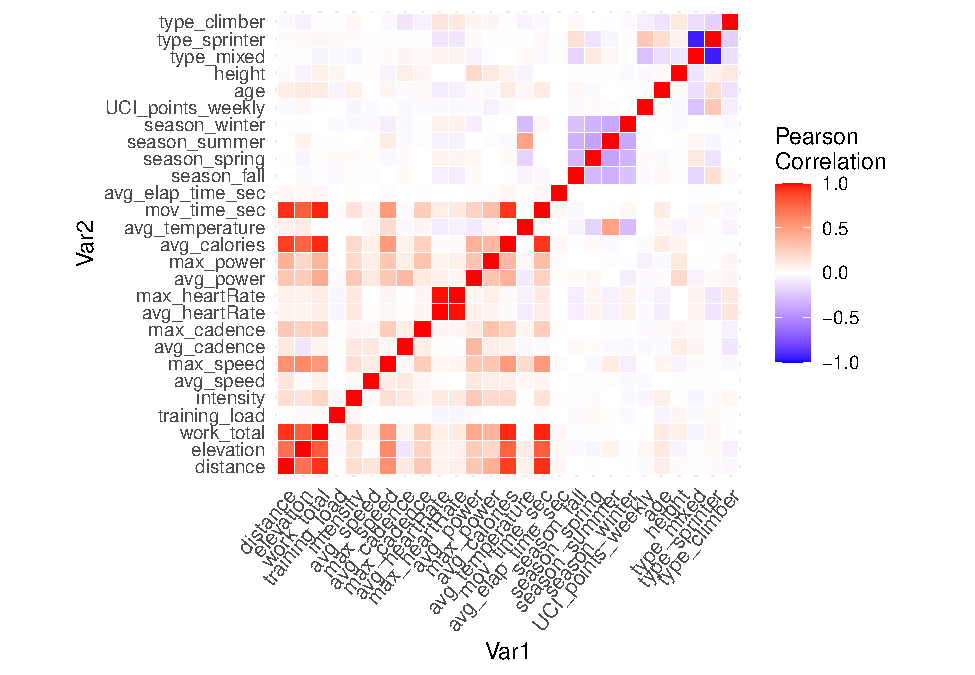
\includegraphics{Master_Thesis_files/figure-latex/heat-map-1} \caption{Heat map for the dataset with average power and dropped NA values.}\label{fig:heat-map}
\end{figure}

Figure \ref{fig:heat-map} shows the Pearson correlation coefficient in a heat map. Tiles which are more reddish implicate a high positive correlation, white tiles implicate that the two variables are uncorrelated while more bluish tiles mark a strong negative correlation. The variables we want to predict are \(avg\_power\) and \(UCI\_points\_weekly\). The variables with the highest correlation for the \(avg\_power\) were \(work\_total\)(0.44), \(avg\_calories\)(0.4) and \(avg\_cadence\)(0.37). For \(UCI\_points\_weekly\) we observed a slightly negative correlation with \(type\_mixed\) and a small positive correlation with \(type\_sprinter\). Therefore we observed that those athletes who focus more on sprint races or tournaments with many sprint sections seemed to achieve higher UCI points, while athletes of \(type\) mixed tended to achieve worse results. The overall low correlation with other variables indicated that a prediction of \(UCI\_points\_weekly\) with the Strava dataset might not achieve good results.

\hypertarget{literature}{%
\section{Literature}\label{literature}}

This section will provide an overview of findings of other authors using ensemble methods to predict average power measurements for professional road cyclists. \textcite{Karetnikov2019} used training data from a professional team and race data from procyclingstats.com to predict a mean maximal power (MMP) attribute for the upcoming race of the two top riders of the professional team. The author aggregated those values choosing several time frames, between 5 and 45 minutes, for the training and race data which were observed by bicycle computers. Another focus was on training and race data in mountainous areas defined as segments above 1500m. A total of 12 prediction techniques, such as LSTM, Decision Trees, Random Forests, XGBoost, CatBoost and 7 different regression models, were used to compare the RMAE as evaluation metrics. The XGBoost model achieved the highest prediction quality of 93\% for the mountain stages and 88\% for the flat stages. While an approach predicting starting positions in races was unsuccessful. A MC-study to identify if the XGBoost and Random Forest tree models depend on the chosen random seed showed that no influence on the prediction quality could be observed.

The research goal of \textcite{Kholkine2020} was to predict race results of the 2018 and 2019 editions of the Tour of Flanders. The authors, approach was to consider the relative finishing time of several races in combination with an ten year exponential moving average and an aggregation of a variety of point achievements such as sprint race points. Team points of each cyclist were gathered from the previous year to account for possible team advantages. \textcite{Kholkine2020} chose XGBoost as the predicting algorithm, since it showed high accuracy in past frameworks and can handle missing values. Imputation was not an option due to the variety of possibilities that an observation is missing. The model predicted 6 riders to be part of the top 10 and 2 cyclists out of top 3 in the 2018 edition correctly but the predicted rank was only correct for one cyclist. The predicted results for 2019 differed heavily from the actual results. No rank was predicted correctly but 4 riders could be properly identified to be part of the top 10. In the end, a comparison to fan prediction showed that the model could beat the fans, predicting expertise in 2018. A feature importance analysis based on the amount of splits each variable was used each time the dataset was divided showed that previous results of the \textit{Omloop Het Nieuwsbald} and the \textit{Tour of Flanders} were key features to the prediction model.

\textcite{Passfield2016} reviewed how power meter output can be evaluated. Several approaches were considered such as smoothing data with a 30 second moving average, mean power output, the maximum mean power output approach, as used by \textcite{Karetnikov2019}, and a critical power model. The latter is defined by a quite intuitive formula \((P-CP)t = W'\). The continuous power output is defined as \(P\), \(CP\) is the critical power, \(t\) is time and \(W'\) is anaerobic capacity. A power output-duration curve can be constructed afterwards. The authors argue that a simple mean power output can be identical for different stressful training or race sessions and therefore does not reflect the variability of power output of each session precisely enough. Furthermore, \textcite{Passfield2016} mention that instead of standard deviation, a detrended fluctuation analysis (DFA) looks more promising to examine power output variability due to its long-range correlations in time-series data.

A comparison between a machine learning model and a mathematical model prediction was made by \textcite{Lemaitre2018}. The authors gradient boosting machine algorithm delivered better prediction results in terms of MAE than the model based on mechanics but stressed that the former had problems to correctly identify short power peaks.

\hypertarget{methods}{%
\section{\texorpdfstring{Methods \label{sec:methods}}{Methods }}\label{methods}}

\hypertarget{regression-trees}{%
\subsection{Regression Trees}\label{regression-trees}}

Decision trees are the most basic tree-based models which are part of the non-parametric algorithms class. The latter means that we do not estimate a direct influence of a variable on the model. The algorithm divides a multi-dimensional feature space into unique sets, so called nodes. Generally, we distinguish between two decision tree tasks, classification and regression trees. Since our \(y\), the variable of interest, \(avg\_power\), \(avg\_power\_weekly\) and \(UCI\_weekly\_points\) are all continuous variables, we will just focus on regression trees. Each split in a regression tree is ruled by the decision of a variable threshold. At the beginning, there is a root node, which contains the entire dataset and implies the first split into subsets. Each following node from a split can be either a decision node or a terminal node. The further term is used for nodes that will lead to a further split of the dataset. If no further split happens at one node, it is called a terminal node, leaf node, leaf. To decide which variable \(x\) and which threshold \(j\) of this variable \(x\) should be chosen to split the dataset, one uses the sum of squared residuals to evaluate the possible splitting decision for a regression trees at a node \(t\).
\begin{equation}
SS_{t} = \sum_i^{n_{1}} (y_1 - \bar{y}_1)^2 + \sum_i^{n_{2}} (y_2 - \bar{y}_2)^2
\end{equation}
with \(y_1 = (y_i|x_i>=j)\), \(y_2 = (y_i|x_i>=j)\). We calculate the \(SS_t\) for each variable \(x\) and each threshold \(j\) of each variable \(x\) of the dataset. Then we chose the variable-threshold combination that generates the lowest \(SS_t\) as our splitting criterion.

\begin{figure}[!H]
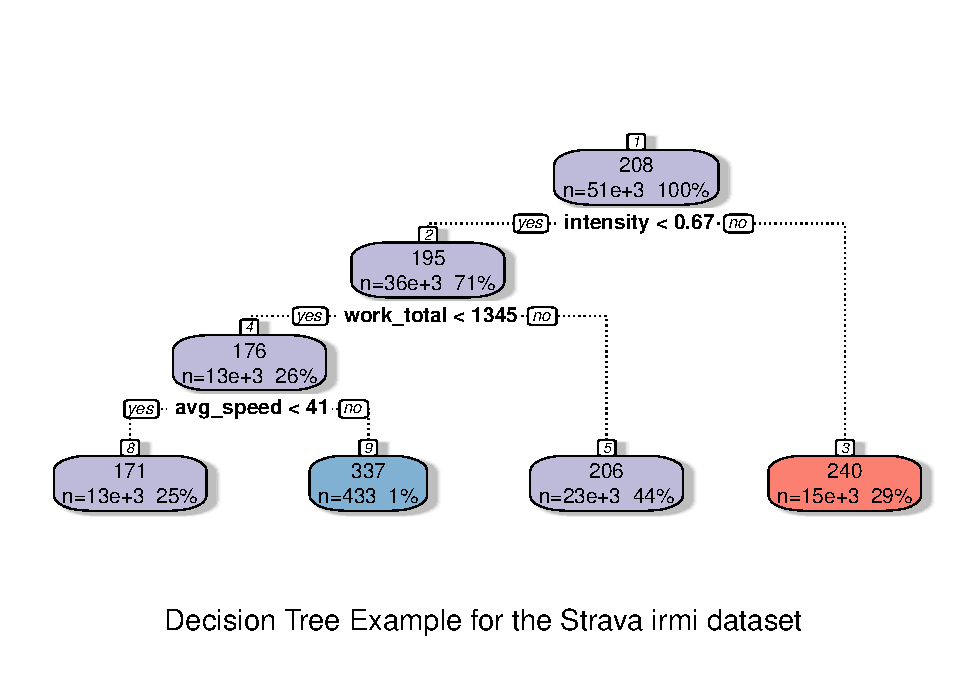
\includegraphics{Master_Thesis_files/figure-latex/decision-tree-1} \caption{Decision Tree Example for the Strava irmi dataset}\label{fig:decision-tree}
\end{figure}

Figure \ref{fig:decision-tree} shows an example of a regression tree with \(y = avg\_power\) and \(X\) containing all variables with a star from \ref{tab:var_list} despite the \(avg\_power\_comb\) variable. In our example, the split at the root node divided the dataset into subsets, that had a value for the variable \(intensity < 0.67\), indicated by \textit{yes}, and those that do not, \textit{no} in the aforementioned figure. The dataset is divided at each decision node, by evaluating all possible thresholds of all variables of the dataset or the subset of the dataset. This procedure is continued, until a further decision would fail to reduce the variance by a specified amount called \textit{complexity parameter}. In figure \ref{fig:decision-tree} this parameter is set to 0.05. So the regression tree only performs a further split if the variance is reduced by at least 5\% in the created node.

\hypertarget{random-forests}{%
\subsection{Random Forests}\label{random-forests}}

Estimating only one decision tree might give us a to narrow solution for the prediction of our target variable. \textcite{Breiman2001} showed that generating several uncorrelated decision trees , in terms of their prediction error, should give on average a better model to predict from than a model from a single tree. This is due to the convergence of the error of the aggregated random forest model. So with an increased number of unique decision trees, the error of the random forest model should converge to the mean average error. To ensure that we aggregate a model of decision trees that have a low correlation between each tree, two methods were used. With bagging, a dataset of \(n\) observations is drawn with replacement from the dataset. Decision trees are very sensitive to (small) changes in the dataset, since decision rules are based on singular values of a variable. If the value of a decision rules is missing, e.g.~due to bagging, a new tree structure is possible, since all subsets after this decision node were affected. The other method is feature subsampling. If we only choose some features of the dataset instead of all and vary those chosen features with each new decision tree, the possibility to end up with an decision tree that is correlated to some other tree from the dataset should be low, and thereby the correlation of the prediction error should be low. To predict the value of the target variable of a new observation, we collect the classification result of each tree in the random forest and choose the class which was predicted by the majority of trees.

\begin{figure}
\centering
\hspace{-3cm}\includegraphics[height = 20cm, width = 20 cm, trim=0in 6in 0in 0.5in,clip]{./includes/RF_pred.pdf}
    \caption{Diagram of a random forest prediction example. A new observation is shown to the model and each tree gives its prediction on the target variable, here $type$, of the Strava dataset. The figure is just for clarification of the concept and does not necessarily represent a possible outcome of a random forest model.  }
    \label{fig:RF_pred}
\end{figure}

Figure \ref{fig:RF_pred} gives an example of a random forest prediction. The latter prediction of the target variable \(type\) would be \(sprinter\), Since 3 out of 4 trees would predict that the new observation would be of type \(sprinter\).

\hypertarget{gradient-boosting}{%
\subsection{Gradient Boosting}\label{gradient-boosting}}

\textcite{Mason1999} proposed an boosting algorithm based on gradient descent. Gradient Boosting Models generate multiple trees and add them together to generate a single ensemble model. The Gradient Boosting machine (GBM) learns with each iteration which the splits worked in terms of a regularized learning objective. Consider some input data \(\{(x_i,y_i)\}^n_{i=1}\) and a differential loss function \(L(y,F(x))\). \(F(x)\) is a model to predict \(\hat{y}\). A loss function is an evaluation metric of a model \(F(x)\) and our target variable \(y\). As an example we will use
\begin{equation}
 L(y,F(x)) = \dfrac{1}{2}(y - \hat{y})^2
 \label{eq:reg_loss}
 \end{equation} as our loss function. Where the \(F(x)\) is a model to predict \(\hat{y}\). The next section \ref{seq:Metrics} will discuss different loss functions. One starts with an initial guess \(F_{0}(x)\) as the prediction of the target variable \(y\), defined as \(\gamma\). Formally
\begin{equation}
 F_{0}(x)=\underset{\gamma}{\operatorname{argmin}} \sum_{i=1}^{n} L\left(y_{i}, \gamma\right)
 \label{eq:ini_val}
 \end{equation} where \({\operatorname{argmin}}\) means that we need to find a \(\gamma\) that minimizes the sum of the equation. Considering the derivative of our loss function, we solve for \(\gamma\) so that
\begin{align}
 \dfrac{\partial L\left(y_{i}, \gamma\right)}{\partial \gamma} &= \dfrac{\partial \sum_{j=1}^n \dfrac{1}{2}(y_j - \gamma)^2}{\partial \gamma} = \sum_{j=1}^n -y_j + \gamma = 0 \\
 \gamma &= \dfrac{\sum_{j=1}^n y_j}{n} = \overline{y}
 \end{align}
the optimal \(\gamma\) for \(F_{y}(x)\) is equal to the mean of \(y\). In other words, the initial prediction \(F_0(x)\) is a leaf, a constant value, that predicts the target variable \(y\). Afterwards, the prediction error \(r\) is obtained as before by subtracting the real value \(y\) from the prediction of the target variable \(\gamma\). So that, for \(m = 1 \quad to \quad M\), where M is the maximum number of trees GBM should build, we compute the prediction errors as
\begin{equation}
 r_{i m}=-\left[\frac{\partial L\left(y_{i}, F\left(x_{i}\right)\right)}{\partial F\left(x_{i}\right)}\right]_{F(x)=F_{m-1}(x)} \text { for } i=1, \ldots, n
 \label{eq:resid_grad_boost}
 \end{equation}. If \(m = 1\) equation \ref{eq:resid_grad_boost} calculates prediction errors for each observation \(i = 1, \ldots,n\) of the dataset for the case of \(F(x) = F_{0}(x)\). Considering the minus in front of the derivative of the latter case, one ends up with \((y -F(x))\), which is equal to the function of a residual. If one uses another loss function, one ends up with a function similar to the residual function but not quite. Therefore, one defines \(r_{i m}\) as pseudo residuals. The gradient in equation \ref{eq:resid_grad_boost} is the reason for the name of GBM. Now the GBM fits a regression tree, but this time instead of predicting the target variable \(y\), we predict the pseudo residuals \(r_{im}\). As before in the Random Forest algorithm, the GBM does not use all possible information of the dataset to build a tree but is restricted by a maximum number of leaf nodes for each tree \(L_m\). So that \(l = 1,\ldots,L_m\) The output values \(\gamma_{l m}\) of each leaf node \(R_{lm}\) are defined as
\begin{equation}
\gamma_{l m}=\underset{\gamma}{\operatorname{argmin}} \sum_{x_{i} \in R_{lm}} L\left(y_{i}, F_{m-1}\left(x_{i}\right)+\gamma\right) \quad l = 1,\ldots,L_m
\label{eq:output_val}
\end{equation} where \(L\left(y_{i}, F_{m-1}\left(x_{i}\right)+\gamma\right)\) is equation \ref{eq:ini_val} expanded by \(F_{m-1}\left(x_{i}\right)\), which defines the previous prediction of the the target variable \(y\). \(\sum_{x_{i} \in R_{lm}}\) defines that only those observations of the dataset were used for the calculation of \(\gamma_{lm}\) that match with the pseudo residuals in leaf \(l\). In the end, due to our chosen loss function, the output values \(\gamma_{lm}\) were always the average of the pseudo residuals in leaf \(l\). In a last step we will update our model with our new predictions so that
\begin{equation}
F_{m}(x)=F_{m-1}(x)+\nu \sum_{j=1}^{m} \gamma_{j m} I\left(x \in R_{j m}\right)
\label{eq:mod_sum}
\end{equation} where \(\nu\) is a learning rate which shrinks the influence of each tree \(m\), so that overfitting is reduced, future trees \(m+1\) can still improve the model and \(\sum_{j=1}^{m} \gamma_{j m} I\left(x \in R_{j m}\right)\) adds up the output value \(\gamma_{lm}\) for all leaves, \(R_{j,m}\) that refer to the pseudo residuals of tree \(m\) and observation \(j\) of the training dataset. GBM will stop building trees and update the pseudo residuals if either the number of trees \(m\) reached the maximum number of trees \(M\) or the shrinkage value of the pseudo residuals \(R_{j,m}\) fall below a specified threshold.

Again we consider the variable \(avg\_power\_comb\) as our target variable. So we calculate the initial prediction value from our target variable, obtain the pseudo residuals as described before and use this pseudo residuals as 4 terminal nodes. Let the 3 splitting rules be \(intensity>0.69\), \(avg\_speed>35.9\) and \(type = mixed\). Then calculate the output value at each leaf node and add the weighted results of this process to each observation of the target variable of each pseudo residual respectively.

\begin{figure}
\centering
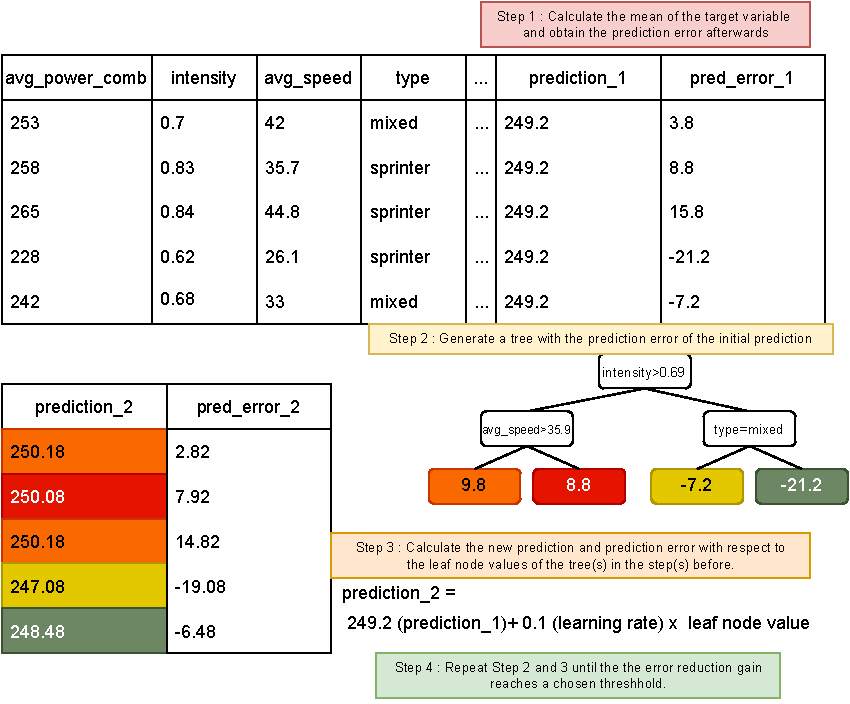
\includegraphics{./includes/grad_boost.pdf}
\caption{The diagram shows exemplary how GBM calculates the predictions.}
\label{fig:grad_boost}
\end{figure}

Figure \ref{fig:grad_boost} shows a visualization of this process. We decided to not include the GBM method in the results section since XGBoost (section \ref{sec:xgboost}) and Lightgbm (section \ref{sec:lgbm}) are direct successors of this technique and are likely to outperform the GBM method. We still included this method to give a good introduction into the following gradient-based tree-ensemble methods.

\hypertarget{xgboost}{%
\subsection{\texorpdfstring{XGBoost \label{sec:xgboost}}{XGBoost }}\label{xgboost}}

The extreme gradient boosting (XGBoost) algorithm was first mentioned by \textcite{Chen2016}.

\begin{equation}
\hat{y}_{i}=\sum_{k=1}^{K} f_{k}\left(\mathbf{x}_{i}\right), \quad f_{k} \in \mathcal{F}
\label{eq:xgboost_pred}
\end{equation}
\begin{equation*}
\text{with }\mathcal{F}=\left\{f(\mathbf{x})=w_{q(\mathbf{x})}\right\}\left(q: \mathbb{R}^{m} \rightarrow T, w \in \mathbb{R}^{T}\right)
\label{eq:tree_space}
\end{equation*}

Equation \ref{eq:xgboost_pred} defines the predicted value \(\hat{y_i}\) as the sum of values from K repetitions of \(f(x_i)\). This means that the prediction of the target value \(y\) for an example \(i\) is given by the sum of predictions from \(K\) trees. \ref{eq:tree_space} from \textcite{Chen2016} shows the space of the regression trees. Let \(T\) be the number of terminal nodes in a tree. Then, \(q\) can be defined as the decision rules which creates the structure of a tree with a root node in the beginning and some terminal nodes in the end. \(w\) can be defined as the continuous score on the \(i\)-th terminal node. So the (final) prediction of \(\hat{y}\) will be calculated by the sum of the corresponding terminal nodes which are given by \(w\). \textcite{Chen2016} expand the loss function of GBM by some regulization paramter \(\Omega\) to create a regularized task.
\begin{equation}
\begin{array}{l}
\mathcal{L}(\phi)=\sum_{i} l\left(\hat{y}_{i}, y_{i}\right)+\sum_{k} \Omega\left(f_{k}\right) \\
\text { where } \Omega(f)=\gamma T+\frac{1}{2} \lambda\|w\|^{2}
\end{array}
\label{eq:reglu_obj}
\end{equation}

In equation \ref{eq:reglu_obj}m the loss function is defined by \(l\left(\hat{y}_{i}, y_{i}\right)\) and calculates the difference of the predicted \(\hat{y}\) and the actual value of \(y\). \(\Omega\) controls the complexity of the model by adding a penalty parameter \(\gamma\) to alter the number of terminal nodes of a tree, and \(\frac{1}{2} \lambda\|w\|^{2}\) is used to level the weights as a protection against overfitting.

To optimize \ref{eq:reglu_obj}, we need to train the model in an additive sense. This means, that in each instance \(i\) of the iteration \(t\) we predict \(\hat{y}_i^{(t)}\) and will add \(f_t\) to minimize the objective. Using an second-order Taylor approximation, we can optimize the objective so that

\begin{equation}
\mathcal{L}^{(t)} \simeq \sum_{i=1}^{n}\left[l\left(y_{i}, \hat{y}^{(t-1)}\right)+g_{i} f_{t}\left(\mathbf{x}_{i}\right)+\frac{1}{2} h_{i} f_{t}^{2}\left(\mathbf{x}_{i}\right)\right]+\Omega\left(f_{t}\right)
\label{eq:gradient_loss}
\end{equation} with
\(g_{i}=\partial_{\hat{y}^{(t-1)}} l\left(y_{i}, \hat{y}^{(t-1)}\right)\) and \(h_{i}=\partial_{\hat{y}^{(t-1)}}^{2} l\left(y_{i}, \hat{y}^{(t-1)}\right)\).
At step \(t\), we can remove \(l\left(y_{i}, \hat{y}^{(t-1)}\right)\) which is independent from \(f(t)\).

\begin{equation}
\tilde{\mathcal{L}}^{(t)}=\sum_{i=1}^{n}\left[g_{i} f_{t}\left(\mathbf{x}_{i}\right)+\frac{1}{2} h_{i} f_{t}^{2}\left(\mathbf{x}_{i}\right)\right]+\Omega\left(f_{t}\right)
\end{equation}

Let \(I_j = \{i|q(x_i) = j\}\) be the instance set of terminal node j. An instance set can be explained as a subset of the dataset with an instance index \(i\) and their gradient statistics \(g_j,h_j\) for each observation \(i\) respectively. Expanding \(\Omega\) in eq. \ref{eq:gradient_loss}, we end up with
\begin{equation}
\begin{aligned}
\tilde{\mathcal{L}}^{(t)} &=\sum_{i=1}^{n}\left[g_{i} f_{t}\left(\mathbf{x}_{i}\right)+\frac{1}{2} h_{i} f_{t}^{2}\left(\mathbf{x}_{i}\right)\right]+\gamma T+\frac{1}{2} \lambda \sum_{j=1}^{T} w_{j}^{2} \\
&=\sum_{j=1}^{T}\left[\left(\sum_{i \in I_{j}} g_{i}\right) w_{j}+\frac{1}{2}\left(\sum_{i \in I_{j}} h_{i}+\lambda\right) w_{j}^{2}\right]+\gamma T
\label{eq:obj_weight}
\end{aligned}
\end{equation}

At the \(t-th\) iteration, we need to sum the weights \(w^2\) of each terminal node. Doing so, we can replace \(f_t(x_i)\) as the function to optimize, with \(w_j\) a parameter to optimize. For each terminal node \(j\), we calculate \(G_j\) and \(H_j\) as the sum of each gradient statistic \(g_i\) and \(h_i\) for each observation \(i\) of the instance set \(I_j\).

Let the structure of \(q(x)\), be fixed, and one can derive the optimal weight \(w^*_j\) of terminal node \(j\), as
\begin{equation}
w_{j}^{*}=-\frac{\sum_{i \in I_{j}} g_{i}}{\sum_{i \in I_{j}} h_{i}+\lambda}
\end{equation}.

\(w_{j}^{*}\) is then used to simplify the regularized learning objective \(\tilde{\mathcal{L}}^{(t)}\) by expanding the object to a function depending on the tree structure \(q\) resulting in
\begin{equation}
\tilde{\mathcal{L}}^{(t)}(q)=-\frac{1}{2} \sum_{j=1}^{T} \frac{\left(\sum_{i \in I_{j}} g_{i}\right)^{2}}{\sum_{i \in I_{j}} h_{i}+\lambda}+\gamma T
\label{eq:score_obj}
\end{equation}.

Equation \ref{eq:score_obj} can be interpreted as a scoring function and thereby as an evaluation metric of the tree structure \(q\). XGBoost uses this function to prune the tree structure \(q\) in the sense that XGBoost chooses the structure \(q\) with the lowest score of \(\tilde{\mathcal{L}}^{(t)}(q)\)

Evaluate each possible split at a decision node, we would often end up with an amount of tree structures \(q\) that is impossible to evaluate. XGBoost therefore uses a greedy algorithm, so that a tree always starts with just the root node and iteratively adds more decision nodes. Let \(I_L\) and \(I_R\) be the instance sets of left and right nodes after a possible splitting decision, with \(I = I_L \cup I_R\). The instance set of a splitting decision can be expressed as the instance set of the left and right node after a possible split. The loss reduction of a possible split candidate can be defined as
\begin{equation}
\mathcal{L}_{\text {split }}=\frac{1}{2}\left[\frac{\left(\sum_{i \in I_{L}} g_{i}\right)^{2}}{\sum_{i \in I_{L}} h_{i}+\lambda}+\frac{\left(\sum_{i \in I_{R}} g_{i}\right)^{2}}{\sum_{i \in I_{R}} h_{i}+\lambda}-\frac{\left(\sum_{i \in I} g_{i}\right)^{2}}{\sum_{i \in I} h_{i}+\lambda}\right]-\gamma.
\label{eq:split_loss}
\end{equation}.

Further methods used to reduce overfitting are shrinkage and column subsampling. Shrinkage scales new weights by a factor \(\eta\) succeeding each step of tree boosting. Thereby the influence of each individual tree is reduced and future trees have a higher possibility to enhance the model, so that one can consider \(\eta\) as a learning rate. Feature subsampling is used to reduce the complexity of each tree structure \(q\). \textcite{Chen2016} propose a weighted quantile sketch algorithm to decrease the computational time needed to find the optimal splitting candidate at each node of the structure \(q\) for each iteration \(t\). The discussion of this technique was omitted as it would go beyond the scope of this thesis.

Figure \ref{fig:xgboost} shows a visualization of the process The implementation of the XGBoost algorithm sets the initial loss \(\mathcal{L}^{(0)} = l(y_i,\hat{y}_i) = 0.5\).
Again we consider the variable \(avg\_power\_comb\) as our target variable. So we calculate the initial prediction value from out target variable,otain the pseudo residuals as described before, and use these pseudo residuals as the dataset for the tree structure \(q\). Let the 3 splitting rules be \(intensity>0.69\), \(avg\_speed>35.9\) and \(type = mixed\). Then calculate the output value at each leaf node and add the weighted results of this process to each observation of the target variable of each pseudo residual respectively.

\begin{figure}
\centering
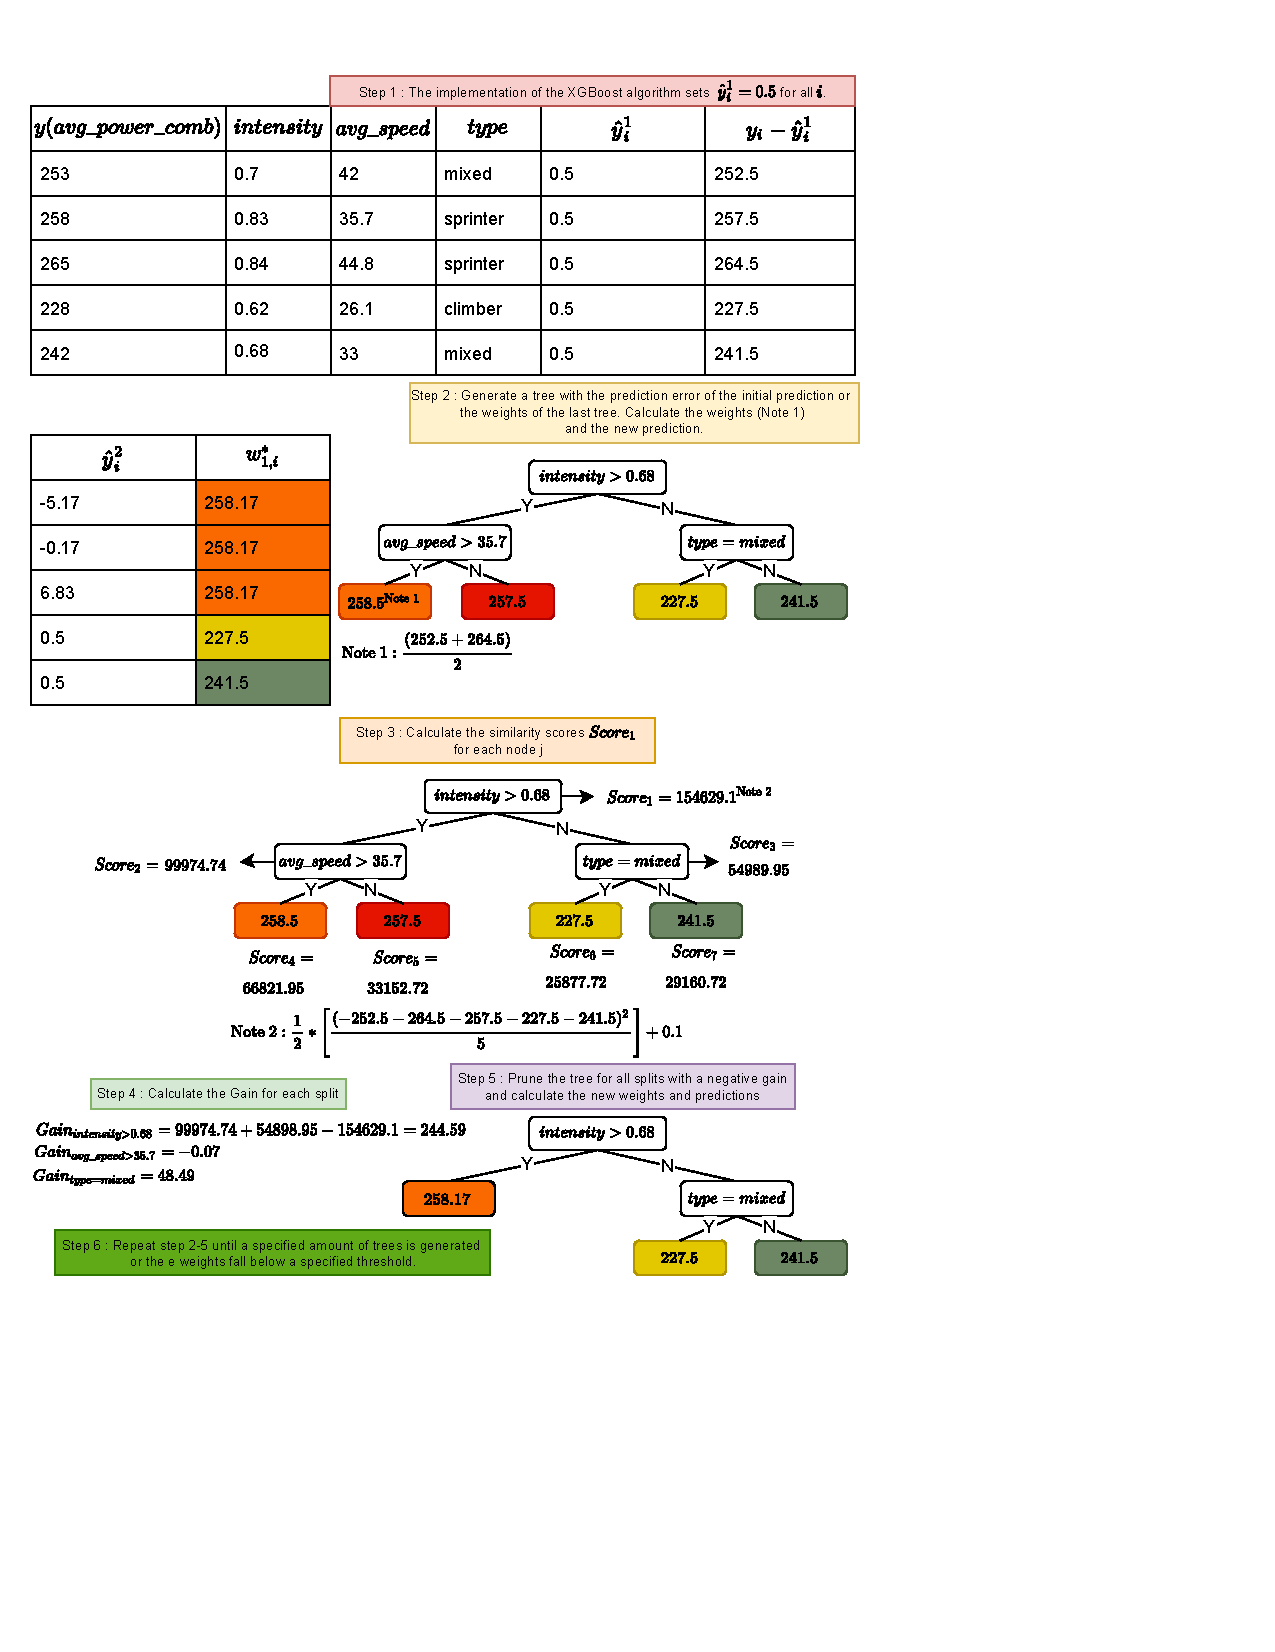
\includegraphics[height = 1.7\linewidth, width = 1.5\linewidth,trim=0.21in 1in 0in 0.0in,clip]{./includes/XGBoost.pdf}
\vspace{-3.6cm}\caption{The diagram shows exemplary how XGBoost initiates the algorithm, builds trees, calculates the weights and updates the model.}
\label{fig:xgboost}
\end{figure}

\hypertarget{lightgbm}{%
\subsection{\texorpdfstring{LightGBM \label{sec:lgbm}}{LightGBM }}\label{lightgbm}}

\textcite{Ke2017} proposed a gradient boosting algorithm called LightGBM (LGBM), which supports a way to differ between instances with small and large absolute gradient statistics. They call this method \textit{Gradient-based One-Side Sampling} (GOSS) and argue that those instances with a small gradient also show a low training error and should therefore receive less attention. GOSS sorts the instances with respect to their absolute value of their gradients in descending order and chooses the top \(l \times 100\%\) instances. From the other \(1-t\) share of instances, GOSS randomly samples \(s \times 100\%\) instances. The latter samples are multiplied with a small weight \(\dfrac{1-l}{s}\) when the loss function is evaluated.

The following explains the splitting decision for trees in LGBM. \(\tilde{v}_{j}(p)\) is the estimated variance gain when we split a feature \(k\) at point \(p\). As explained before, LGBM differs between instances with large and small absolute gradient statistics. So that \(C_l = \left\{x_{i} \in C: x_{i k} \leq p\right\}\), \(C_{r}=\left\{x_{i} \in C:x_{ik}>p\right\}\). The feature values smaller than or equal to the threshold \(p\) of those instances with large absolute gradient statistics would be split to the left child node and those exceeding the threshold \(p\) would be split to the right child node. The same definition holds for \(D_l\) and \(D_r\), with the difference that \(D\) represents randomly sampled instances from those with already low absolute gradient statistics. Formally, LGBM estimates \(\tilde{v}_k(p_k^*)\), because we train with a dataset of instances that is smaller than the dataset of all possible instances, such that
\begin{equation}
\tilde{v}_{j}(p)=\frac{1}{n}\left(\frac{\left(\sum_{x_{i} \in C_{l}} g_{i}+\dfrac{1-l}{s} \sum_{x_{i} \in D_{l}} g_{i}\right)^{2}}{n_{l}^{k}(d)}+\frac{\left(\sum_{x_{i} \in C_{r}} g_{i}+\dfrac{1-l}{s} \sum_{x_{i} \in D_{r}} g_{i}\right)^{2}}{n_{r}^{k}(pd)}\right).
\label{eq:lgbm_split}
\end{equation}

Due to the lower amount of instances, LGBM reduces the computation time to find the best split candidate at each decison node.
The other important difference of LGBM compared to XGBoost is exclusive feature bundling. Consider a sparse dataset with many dummy features, such that their distribution is binary. \textcite{Ke2017} argued that those many features in a dataset with a sparse feature space are mutually exclusive, e.g.~features that never share nonzero values for all observations. LGBM stacks those features into one feature \textit{bundle} and thereby reduces the dataset dimension from \(\mathop{\#data} \times \mathop{\#features}\) to \(\mathop{\#data} \times \mathop{\#bundle}\) with \(\mathop{\#bundle}<<\mathop{\#features}\). This reduces the time to find splits since less features have to be considered.

\hypertarget{catboost}{%
\subsection{\texorpdfstring{Catboost \label{seq:catboost}}{Catboost }}\label{catboost}}

\textcite{Prokhorenkova2019} proposed an enhanced gradient boosting algorithm called CatBoost. The latter is an abbreviation for categorical boosting. They claim to be the first, who found a solution to the problem of target leakage in gradient boosting. The latter implies that due to the usage of the same training observations, for the calculation of the gradient statistics and models used to minimize those gradients, a prediction shift is produced. They also found a similar problem with the encoding of categorical variables which will be explained at the end of this section.

Considering a dataset \(\mathcal{D}\) as described before for XGBoost, CatBoost wants to minimize the expected loss \(\mathcal{L}(F):=\mathbb{E} L(y, F(\mathbf{x}))\) through an iteratively updated object \(F\). The latter object will be approximated by \(F^t\) with \(t = 0,1,\ldots\) through the gradient boosting procedure as explained in GBM and XGBoost. Given that \(h^t\) is a function for a binary decision tree, as we minimize the expected loss by

\begin{equation}
h^{t}=\underset{h \in H}{\arg \min} \ \mathcal{L}\left(F^{t-1}+h\right)=\underset{h \in H}{\arg \min } \mathbb{E} L\left(y, F^{t-1}(\mathbf{x})+h(\mathbf{x})\right).
\end{equation}

Catboost takes the (negative) gradient step instead of the second-order Taylor approximation to solve the minimization problem, so that \(h^t\) approximates \(-g^t(\mathbf{x},y)\), with \(g^{t}(\mathbf{x}, y):=\left.\frac{\partial L(y, s)}{\partial s}\right|_{s=F^{t-1}(\mathbf{x})}\). \textcite{Prokhorenkova2019} then use a least-squares approximation so that:

\begin{equation}
h^{t}=\underset{h \in H}{\arg \min } \mathbb{E}\left(-g^{t}(\mathbf{x}, y)-h(\mathbf{x})\right)^{2}
\label{eq:grad_boost_exp}
\end{equation}

Equation \ref{eq:grad_boost_exp} shows the ideal way to approximate \(h^t\), but since we cannot know the expectation, an approximation often uses the same dataset \(\mathcal{D}\) so that :

\begin{equation}
h^{t}=\underset{h \in H}{\arg \min } \frac{1}{n} \sum_{k=1}^{n}\left(-g^{t}\left(\mathbf{x}_{k}, y_{k}\right)-h\left(\mathbf{x}_{k}\right)\right)^{2}
\end{equation}

The authors now argue that the aforementioned prediction shift is due to a shift in \(g^{t}\left(\mathbf{x}_{k}, y_{k}\right)| \ \mathbf{x}_{k}\) from \(g^t(\mathbf{x},y)|\ \mathbf{x}\), since \(F^t\) was trained using \(y_k\). This implies that h\^{}t is a biased estimate of \(\hat{y}^t\) which leads to a bias in \(F^T\), since the target values \(y_k\) of the same observations were used for all curent models \(F^{t-1}\).
As in equation \ref{eq:mod_sum} of GBM, CatBoost updates its prediction model in an iterative sense. The authors argue that this bias comes from a ``shift of the conditional distribution \(F\left(\mathbf{x}_{k}\right) \mid \mathbf{x}_{k} \text { for a training example } \mathbf{x}_{k} \text { from the distribution of } F(\mathbf{x}) \mid \mathbf{x} \ \text {for a test example } \mathbf{x}\).'' Due to the latter, the learned model suffers from a (prediction) shift, so \(F(\hat{y_k}|y_k)\) is shifted. CatBoost solves this by a technique called Ordered Boosting.

Let \(I\) be the amount of trees a model is learned with. Unshifted residuals \(r^{I-1}(\mathbf{x_k},y_k)\) can only obtained if we exclude observation \(\mathbf{x}_k\) in the training process of \(F{I-1}\). The authors argue that the training process would become impossible because, since all residuals need to be unshifted, we cannot use any observations for the training process of \(F{I-1}\). \textcite{Prokhorenkova2019} solve this by a set of models which doe not include any information of the predicted observation. Therefore, one uses a permutation \(\sigma\) of \(\mathcal{D}\) and learns \(n\) unique models \(M_1,\ldots,M_n\). Each model \(M_i\) uses only observations in the permutation \(\sigma\) between the first and and the \(i\)-th observation. The residual of the \(j\)-th observation in the permutation \(\sigma\) uses the model \(M_{j-1}\). CatBoost combines the latter method with gradient boosting with symmetrical decision trees to obtain unbiased residuals \(R(\mathbf{x}_k,y_k)\) and thereby an unbiased combined model \(F\).

Figure \ref{fig:ordered_boost} shows how the ordered boosting algorithm works to create the combined model \(F\). Since the calculation of the residuals and the iterative manner of gradient boosting techniques were explained in detail for GBM and XGBoost, figure \ref{fig:ordered_boost} focuses more on the unique differences to other gradient boosting techniques.

\begin{figure}
\centering
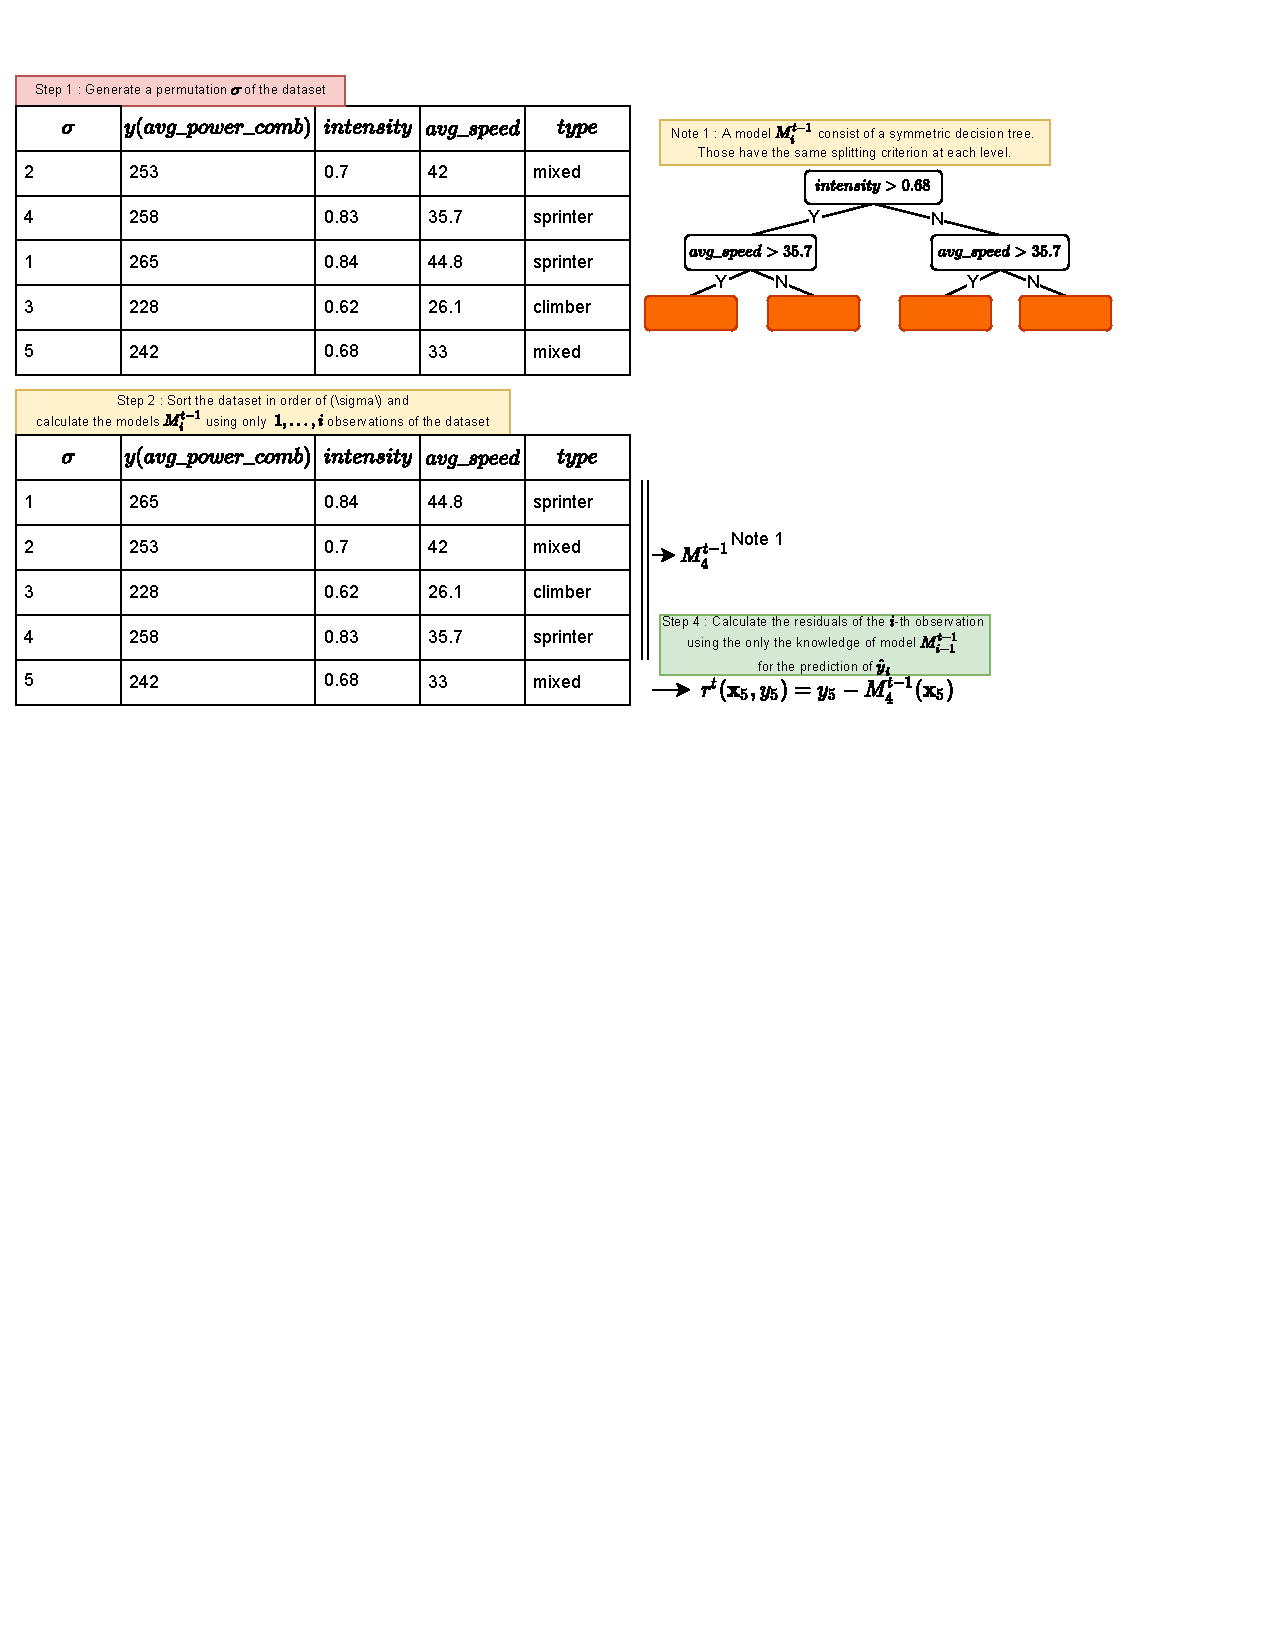
\includegraphics[height = 1.7\linewidth, width = 1.1\linewidth,trim=0in 4.7in 0in 0.0in,clip]{./includes/Ordered_Boosting.pdf}
\vspace{-3.6cm}\caption{The diagram shows how the orderd boosting algorithm in CatBoost works.}
\label{fig:ordered_boost}
\end{figure}

Categorical features have often been encoded by one-hot-encoding. This means splitting the (categorical) feature specifications by adding new binary variables. This can lead to a sparse dataset due to the large expansion of the feature space, if the categorical features have a high cardinalty, e.g.~a userID feature. \textcite{MicciBarreca2001} proposed to tackle this problem using target statistics which estimates the expected target value for each feature specification, thereby grouping categories and using the target statistic as a new numerical variable instead. \textcite{Prokhorenkova2019} claim that the prediction shift mentioned before applies in the same way when computing target statistics for a categorical feature. To avoid this, they propose a sub-sampling so that \(\mathcal{D}_{k}\subset\mathcal{D}_{\left\{\mathbf{x}_{k}\right\}}\) is used to calculate the target statistics for \(x_k\), therefore excluding \(x_k\) from the process. Let \(p\) be some prior to smooth the estimate \(\mathbb{E}(y|x^i=x^i_k)\) for categories of a feature with a low proportion compared to the other categories of that feature, then :
\begin{equation}
\hat{x}_{k}^{i}=\frac{\sum_{\mathbf{x}_{j} \in \mathcal{D}_{k}} \mathbb{1}_{\left\{x_{j}^{i}=x_{k}^{i}\right\}} \cdot y_{j}+a p}{\sum_{\mathbf{x}_{j} \in \mathcal{D}_{k}} \mathbb{1}_{\left\{x_{j}^{i}=x_{k}^{i}\right\}}+a}
\label{target_stat_cat}
\end{equation}

\textcite{Prokhorenkova2019} then introduce a technique called ordered targeting statistic. Comparable to the online learning algorithm, we feed the model sequentially, using a random permutation \(\sigma\) of the training dataset. Thereby, the model observes in each iteration another new training observation of the permuted training dataset, but all other observations from past iterations will be used to compute the target statistic as well. More formally, for the training process, equation \ref{target_stat_cat} will use \(\mathcal{D}_{k}=\left\{\mathbf{x}_{j}: \sigma(j)<\sigma(k)\right\}\), and for testing, one uses the whole dataset \(\mathcal{D}_{k}=\mathcal{D}\).

\begin{table}[!htbp]
\centering
\scriptsize
\captionsetup{labelsep=newline, justification=centering}
  \begin{threeparttable}
       \caption{\textit{Orderd Target Statistics Example}}
     \begin{tabular}{*{5}{l}}
        \toprule
         \multicolumn{1}{l}{\makecell{\textbf{ target}}}& \multicolumn{1}{l}{\makecell{\textbf{ target}}} & \multicolumn{1}{c}{\makecell{\textbf{encoded target}\\ \textbf{prior p = 0.05, a = 1}}} & \multicolumn{1}{l}{\makecell{\textbf{history}}} & \multicolumn{1}{l}{\makecell{\textbf{ explanation}}} \\
        \midrule
         \multicolumn{1}{l}{\makecell{0}}& \multicolumn{1}{l}{\makecell{mixed}} & \multicolumn{1}{c}{\makecell{$\frac{0+0.05}{0+1} = 0.05$}} & \multicolumn{1}{l}{\makecell{1}} & \multicolumn{1}{l}{\makecell{$\frac{\text{No \textit{mixed} with target = 1 in history + a$\times$prior}}{\text{No \textit{mixed} in history + a }}$}} 
 \\
         \multicolumn{1}{l}{\makecell{1}}& \multicolumn{1}{l}{\makecell{sprinter}} & \multicolumn{1}{c}{\makecell{ $\frac{0+0.05}{0+1}=0.05$}} & \multicolumn{1}{l}{\makecell{2}} & \multicolumn{1}{l}{\makecell{$\frac{\text{No \textit{sprinter} with target = 1 in history + a$\times$prior}}{\text{No \textit{sprinter} in history + a }}$}} \\
 \\
         \multicolumn{1}{l}{\makecell{1}}& \multicolumn{1}{l}{\makecell{mixed}} & \multicolumn{1}{c}{\makecell{ $\frac{0+0.05}{1+1}=0.025$}} & \multicolumn{1}{l}{\makecell{3}} & \multicolumn{1}{l}{\makecell{$\frac{\text{No \textit{mixed} with target = 1 in history + a$\times$prior}}{\text{One\textit{mixed} in history + a }}$}} 
 \\
         \multicolumn{1}{l}{\makecell{0}}& \multicolumn{1}{l}{\makecell{climber}} & \multicolumn{1}{c}{\makecell{ $\frac{0+0.05}{0+1}=0.05$ }} & \multicolumn{1}{l}{\makecell{ 4}} & \multicolumn{1}{l}{\makecell{$\frac{\text{No \textit{climber} with target = 1 in history + a$\times$prior}}{\text{No \textit{climber} in history + a1 }}$}} 
 \\
         \multicolumn{1}{l}{\makecell{1}}& \multicolumn{1}{l}{\makecell{mixed }} & \multicolumn{1}{c}{\makecell{ $\frac{1+0.05}{2+1}=0.35$ }} & \multicolumn{1}{l}{\makecell{ 5}} & \multicolumn{1}{l}{\makecell{$\frac{\text{One \textit{mixed} with target = 1 in history + a$\times$prior}}{\text{Two \textit{mixed} in history + a }}$}} 
\\
        \bottomrule
     \end{tabular}
      \label{tab:ordered_ts}
  \end{threeparttable}
\end{table}

Table \ref{tab:ordered_ts} shows a less formal explanation of ordered target statistics. Consider each row of \textit{target} and \textit{type} as single observations of the exemplary dataset. The derivation of the value in column \textit{encoded target} is explained in the column \textit{explanation}. The column \textit{history} describes the `observed history' of the ordered target statistics calculation. Such that, for the value of row with \(history = 3\), we have \(target = 1\) and \(type = mixed\). No `observed history' exists with \(target = 1\), and \(type = mixed\), so \(\sum_{\mathbf{x}_{j} \in \mathcal{D}_{k}} \mathbb{1}_{\left\{x_{j}^{i}=x_{k}^{i}\right\}} \cdot y_{j}+a p\) in equation \ref{target_stat_cat} is still 0, but \(\sum_{\mathbf{x}_{j} \in \mathcal{D}_{k}} \mathbb{1}_{\left\{x_{j}^{i}=x_{k}^{i}\right\}}\) is now 1 since the sum of the denominator is no conditioned on the target value \(y_j\). The latter is important, since \textcite{Prokhorenkova2019} argue that a desired property of the target statistics feature calculation and the learning process of the model is the effective usage of all training data. Still, the oblivious counter of the fraction satisfies the requirement to counter the prediction shift. The authors called this bias target leakage, since recognizing the actual target value of the observation for which the \textit{encoded target} calculation is performed, leaks information about the distribution of the target to the encoding process. Since this learned distribution might differ from the distribution of the target value in the test dataset, a biased prediction due to overfitting is possible.

\hypertarget{hyperparameter-optimization}{%
\subsection{Hyperparameter Optimization}\label{hyperparameter-optimization}}

To optimize the tree ensemble models we can optimize their hyperparameters. This subsection will introduce four hyperparameter optimization (HPO) methods and discuss the choice for this work. Furthermore, we will discuss which hyperparameters are possible and useful for each tree ensemble technique.
Tree ensemble algorithm such as the gradient boosting tree implementations of XGBoost, Lightbm and Catboost have several hyperparameter which handle :

\begin{itemize}
\item \textbf{learning rate} - the contribution of each (tree) model, often a factor betwen 0 and 1
\item \textbf{mtry}  - defines how many variables will be used for each (tree) model
\item \textbf{sample size} - defines the number or share of observations of the training dataset to be used in each (tree) model 
\item \textbf{tree depth} - the maximum amount of levels each tree can generate
\item \textbf{trees} - the number of trees to build
\item \textbf{minimal node size} - a minimum number of observations in a node needed to accept a new split at a decision node of a tree 
\item \textbf {loss reduction} - minimum loss reduction needed to accept a split at a decision node of a tree 
\item \textbf{iteration stop} - the number of trees without improvement before stopping the algorithm 
\end{itemize}

The aim of HPO is to find a set of hyperparameter values for a (machine learning) method which minimizes the chosen loss function to evaluate the quality of the model on the validation dataset. Let the chosen loss function be some function \(f(x)\) and \(x^*\) the set of optimal hyperparameter values, then HPO can be stated as :
\begin{equation}
x^* = \underset{x \in \mathcal{X}}{\arg \min }f(x)
\label{eq:HPO}
\end{equation}

\hypertarget{manual-search}{%
\subsubsection{Manual search}\label{manual-search}}

The most simple solution for HPO is to choose a parameter value for each hyperparameter and compare the result of the loss function to some other parameter values. This is repeated until a reasonable low loss function value is found.

\hypertarget{grid-search}{%
\subsubsection{Grid search}\label{grid-search}}

Grid search uses a user specified vector of possible values for each hyperparameter to be tuned. Then all possible combinations of hyperparameter values are evaluated and the combination with the lowest metric value is chosen. This leads to a large amount of possible combinations to evaluate and therefore to a possible long computation time while at the same time only finding a solution for values specified by the user.

\hypertarget{random-search}{%
\subsubsection{Random search}\label{random-search}}

This HPO method do not uses any kind user specification for the hyperparameter values. Random search randomly samples hyperparameter values from the range of each hyperparameter sets, evalutes them and continues until a specified amount of iterations is reached. The hyperparameter set which accomplished the lowest metric value is retunred.

\hypertarget{bayesian-hpo}{%
\subsubsection{Bayesian HPO}\label{bayesian-hpo}}

\textcite{Bergstra2012} argue that the latter two methods show slightly better performance in terms of loss reduction per computational time than manual search. Still, both suffer from the problem that they cannot evaluate the chosen set of hyperparameter values after each iteration. This problem is solved by Bayesian HPO which uses an acquisition function as a prior for the hyperparameter set to evaluate next. Consider an objective function such as equation \ref{eq:reglu_obj} from XGBoost and a dataset with \(n\) observations and \(d\) features, which are the hyperparameters of our objective function, so that \(x_i = (x_{i1},\ldots,x_{id})^T\) and \(y_i = y_i(x)\) Either one initialize the optimization process with \(t\) hyperparameter sets with \(t\in n\) or the algorithm randomly samples \(t\) of such sets w.r.t. the range of each hyperparameter. \(D_0 = {x_1,\ldots,x_n}\) stores the hyperparameter sets for \(n\) trials in a \(n \times d\) matrix \(X\). Normalization of \(x_i\) achieves \(x_i \in [0, 1]^d\). Afterwards, each set \(i\) is used with the objective function to obtain a performance metric as the \(i\)-th observation of the dependent variable \(y_i\). Those outputs are stored in the \(n \times 1\) vector \(Y = y(X) = (y_1,\ldots,y_n)^T\). Instead of continuing to evaluate the objective function for further hyperparameter sets, Bayesian HPO uses a surrogate model to estimate the function to be optimized. The model used in this implementation is the Gaussian Process (GP) model:

\begin{equation}
y\left(x_{i}\right)=\mu+z\left(x_{i}\right) ; \quad i=1, \ldots, n
\label{eq:GP_model}
\end{equation}
where \(\mu\) is the overall mean and \(z(x_i)\) defines the GP with \(E[z(x_i)] = 0\), \(Var[z(x_i)]=\sigma^2\) and \(Cov(z(x_i),z(x_j))= \sigma^1R_{i,j}\). Let \(y(X) \sim N_{n}\left(\mathbf{1}_{\mathbf{n}} \mu, \Sigma\right)\), where \(N_{n}\left(\mathbf{1}_{\mathbf{n}} \mu, \Sigma\right)\) is a multivariate normal distribution with \(\Sigma=\sigma^{2} R\) defined through a correlation matrix \(R\) with elements \(R_{ij}\) and \(\mathbf{1}_{\mathbf{n}}\), a vector of length \(n\) with all ones s \(n\times 1\). The algorithm uses the Gaussian correlation function from \textcite{Ranjan2011}:

\begin{equation}
R_{i j}=\prod_{k=1}^{d} \exp \left\{-\theta_{k}\left|x_{i k}-x_{j k}\right|^{2}\right\}, \quad \text { for all } i, j
\end{equation} with \(\theta = (\theta_1,\ldots,\theta_d \in [0,\infty)^d\) defines a vector for the values of a hyperparameter set. Less formal, the GP estimates a function to model the hyperparameter sets and their estimated metric value. With \(\Sigma\) defines a confidence interval for this estimated function which covers a larger area where the function estimate is only given by very few observations and covers a smaller area where more observations were sampled so far. Thus we can say that a larger confidence interval implies a higher uncertainty of the actual function values in this area.

\begin{figure}[!H]
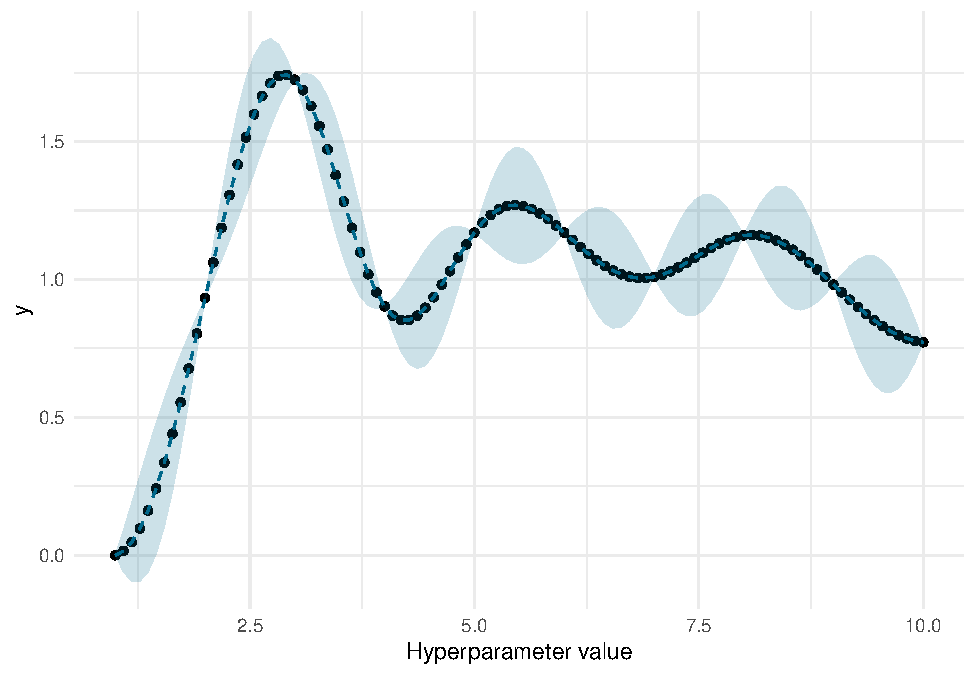
\includegraphics{Master_Thesis_files/figure-latex/baysianHPO-1} \caption{Examplary Gaussian Process for a single Hyperparameter}\label{fig:baysianHPO}
\end{figure}

\ref{fig:baysianHPO} show an exemplary GP which was generated by predicting 100 possible candidates between 1 to 10 for the hyperparameter value \(x\) and evaluated them using an arbitrary evaluation function \(y\), defined by equation \ref{eq:gp_y}.
\begin{equation}
y = \dfrac{a + (\sum_{i=1}^k b_i)^2 - 0.69 \times a ^3 + log(x) }{2 \times a + log(x)}
\label{eq:gp_y}
\end{equation} with \(a = \mathcal{U}(1, 10)\) being a random variable drawn from the uniform distribution between 1 and 10 and \(b = \mathcal{N}(0,0.5^2)\) beeing a random variable drawn from the normal distribution with mean \(0\) and variance of \(0.5^2\). We observe that the confidence bound increases in size, the greater the distance between two candidates who have already been evaluated. Considering that our goal would be the hyperparameter value that minimizes the evaluation function value the GP would continue sampling values around \(x = 4\) and probably between \(x=9\) and \(x = 10\) since we would expect here the largest reduction in terms of the evaluation function given the estimated confidence bound.

The next step of the algorithm is to sample and evaluate new possible hyperparameter sets for the objective function. The GP helped to reduce the evaluation time as the process can estimate metric outcomes with some uncertainty. To take the decision which hyperparameter set should be evaluated next with the actual objective function, the Bayesian HPO algorithm uses an acquisition function. The output of this function told us which hyperparameter set \(x\) is the most promising to evaluate next with the objective function for the underlying model. Possible candidates for the acquisition functions are the lower (minimization)/upper (maximization) confidence bound or the probability of improvement and the expected improvement (EI) \textcite{Wilson2018}. The implementation of the Bayesian HPO used in this thesis was the EI. The EI is defined as
\begin{equation}
E I(\mathbf{x})=\mathbb{E}[\max (0, f(\mathbf{x})-f(\hat{\mathbf{x}}))]
\label{eq:exp_imp}
\end{equation} where \(f(x)\) is the GP estimation of our underlying model metric with hyperparameter set \(x\), and \(f(\hat{x})\) is the best performance that we have tried so far, since the GP is modelling a function of the probability of the model's metric dependent on the hyperparameter set \(x\). For any set of \(X\), we generate a normal distribution for the prediction of the value of \(f\), such that :

\begin{equation}
p(f(\mathbf{x}) \mid \mathbf{x}) \sim \mathcal{N}(\mu(\mathbf{x}), \sigma(\mathbf{x})).
\label{eq:prob_distr_GP}
\end{equation}

Following \textcite{Brochu2010}, one integrates the probability distribution from equation \ref{eq:prob_distr_GP} multiplied with the difference of the performance from the hyperparameter set on trial and the best hyperparameter set so far. This leads to

\begin{equation}
\begin{aligned}
E I(\mathbf{x}) &=\int_{f(\hat{\mathbf{x}})}^{\infty} p(f(\mathbf{x}) \mid \mathbf{x})(f(\mathbf{x})-f(\hat{\mathbf{x}})) d f(\mathbf{x}) \\
&=\int_{f(\hat{\mathbf{x}})}^{\infty} \mathcal{N}(f(\mathbf{x}) \mid \mu(\mathbf{x}), \sigma(\mathbf{x}))(f(\mathbf{x})-f(\hat{\mathbf{x}})) d f(\mathbf{x}) \\
&= (\mu(\mathbf{x})-f(\hat{\mathbf{x}})) \Phi(z)+\sigma(\mathbf{x}) \phi(z)
\end{aligned}
\end{equation}
with \(\phi\) defining the probability density function of the standard normal, \(\Phi\) being the cumulative distribution function of the standard normal distribution, while z is defined as the difference between the GP mean and the best performance so far scalled by the standard deviation of the GP. Formally
\begin{equation}
z=\frac{\mu(\mathbf{x})-f(\hat{\mathbf{x}})}{\sigma(\mathbf{x})}.
\end{equation}

The GP estimated \(\mu(x)\) and \(\sigma(x)\) that helped us to find the \(x\), which we believe gives us the best EI for our next sample of \(x\)
\begin{equation}
\mathbf{x}_{t+1}=\arg \underset{\mathbf{x}_{t+1}}{\min } E I\left(\mathbf{x}_{t+1}\right).
\end{equation}
Thereby, the Bayesian HPO creates a balance between exploring uncertain hyperparameters (exploration) and gathering observations from hyperparameters near the optimum (exploitation) \textcite{Snoek2012}.
The algorithm stops after a user defined number of rounds without an positve expected improvement on the models metric.

\hypertarget{hyperparameter-of-tree-ensemble-models}{%
\subsubsection{Hyperparameter of tree ensemble models}\label{hyperparameter-of-tree-ensemble-models}}

In this subsection we will discuss the hyperparameter of the Random Forest, GBM, XGBoost, Light Gradient Boosting and CatBoost methods used in this thesis.

\hypertarget{random-forest}{%
\subsubsection{Random Forest}\label{random-forest}}

Random Forest is cited by several publications as a model which performs good with default parameters, i.e.~without tuning \textcite{Shahhosseini2019}. Additionally, there are many hyperparameter to tune compared to gradient boosting based models like XGBoost.
The main hyperparameters for a random forest model are \textit{mtry} and \textit{minimal node size}, which are defined ,in the algorithm used in this thesis, as \textit{mtry} and \(min\_n\) respectively.

\hypertarget{gradient-boosting-methods}{%
\subsubsection{Gradient Boosting methods}\label{gradient-boosting-methods}}

The gradient boosting method implementations of GBM,XGBoost,LightGBM and CatBoost used in this paper feature different hyperparameters to tune as shown in table \ref{tab:hyperparameter}.
The \textit{trees} hyperparameter is usually not tuned but fixed for a specific value, e.g.~in \textcite{Wang2020} and \textcite{Karetnikov2019}.

\begin{table}[!htbp]
\centering
\scriptsize
\captionsetup{labelsep=newline, justification=centering}
  \begin{threeparttable}
       \caption{\textit{Hyperparameter tuned for each method}}
     \begin{tabular*}{ \linewidth}{{l@{\extracolsep{\fill}}cr}}
        \toprule
         \multicolumn{1}{l}{\textbf{ Parameter}}& \multicolumn{1}{c}{Model} & \multicolumn{1}{c}{Range} \\
        \midrule
        \addlinespace
        \textbf{tree depth} & All &  [1,100]\\ 
        \addlinespace
        \textbf{mtry (see table notes)} & All &  [0,25]\\ 
        \addlinespace
        \textbf{learning rate} & XGBoost, LightGBM, Catboost &  [0,1]\\ 
        \addlinespace
        \textbf{loss reduction} &  XGBoost, LightGBM    &  [0,$\infty$]\\ 
        \addlinespace
        \textbf{tree depth} &  XGBoost ,LightGBM, Catboost  &  [1,$\infty$]\\ 
        \addlinespace
        \textbf{minimal node size} &  XGBoost, LightGBM, Catboost   &  [1,$\infty$]\\ 
        \bottomrule
     \end{tabular*}
    \begin{tablenotes}[flushleft]
      \small
      \item \textit{Note: The upper bound of the hyperparameter \textit{mtry} differs due to the chosen method. This was up to 25 for Random Forest and XGBoost and Lightgbm models. Catboost models, which uses ordered target statistics to encode \textit{factor} variables, had only up to 22 variables. The latter, as explained in the section \ref{seq:catboost}, do not expand the dataset but encode the variable itself.} 
    \end{tablenotes}
      \label{tab:hyperparameter}
  \end{threeparttable}
\end{table}

\hypertarget{metrics}{%
\subsection{\texorpdfstring{Metrics \label{seq:Metrics}}{Metrics }}\label{metrics}}

Metrics, in modeling applications, are functions to evaluate and compare the performance of models. Such metrics are also used as a loss function in gradient boosting methods to evaluate each (tree) model performance. A recent review study on machine learning results in team sports by \textcite{Claudino2019a} could not come up with a specific metric of choice but named those which achieved the best results in their sport. \textcite{Tofallis2015} mentioned as well that there is still not a specific metric of choice. Furthermore, they stress that there is no law for studies to just stick to one metric and added that each prediction method stores another piece of information. Therefore, this section will look into several prediction metrics for model selection with respect to former sports and especially, road cycling prediction results and benefits for our chosen methods.

\begin{equation}
RMSE = \sqrt{\dfrac{\sum^{n}_{t=1} (\hat{y}_t-y_t)^2}{n}} 
\end{equation}
where \(y_t\) is the is the \(t^{th}\) real observation of the dataset, \(\hat{y_t}\) is the \(t^{th}\) predicted observation of the dataset
and \(n\) is the total number of observations of the dataset. The RMSE is a more favorable metric when it comes to machine learning algorithm compared to of the MAE. This is due to the gradient of the RMSE of the \(t^{th}\) prediction which differs from that of the MSE.

\begin{equation}
\dfrac{\delta RMSE}{\delta y_n}=\dfrac{1}{2}\dfrac{1}{\sqrt{MSE}}\dfrac{\delta\text{MSE}}{\delta y_n} 
\label{eq:RMSE_2}
\end{equation}
In equation \ref{eq:RMSE_2}, we can see that gradient of the RMSE gives more weight to larger errors, which can be preferable if the dataset has many outliers.

\begin{equation}
MAE = \dfrac{1}{n}\sum^n_{t=1}\big|y_t-\hat{y}_t\big|
\end{equation}
The mean average error (MAE) is a quite simple metric but faces two main drawbacks. First, since the MAE is measured on the same scale as the data, the error can be biased due to different scales of the dataset variables.

\begin{equation}
MAPE = \dfrac{1}{n}\dfrac{\sum^n_{t=1} \big|y_t-\hat{y}_t\big|}{y_t}
\end{equation}
The mean absolute percentage error (MAPE), sometimes referred to as mean magnitude of relative error (MMRE), is widely used in businesses and organizations \textcite{Tofallis2015}, as well as in football \textcite{Strnad2015} and professional road cycling performance prediction \textcite{Karetnikov2019}. \textcite{Tofallis2015} showed that, in regression tasks, the MAPE metric will tend to under-predict the forecast. The latter means that for the same error is higher when \(\hat{y}_t<f_n\) compared \(\hat{y}_t>f_n\). The advantage of this metric is the intuitive interpretation compared to the RMSE. That is because the latter presents us an absolute value which needs specific knowledge of the field to decide if the forecast can beat other forecasting methods such as an expert's guess

The coefficient of determination better known as \(R^2\) is the relative amount of the variation in the target variable \(y\) that is predictable from the dependent variable matrix \(X\) with \(y\) a \(n \times 1\) vector with \(n\) observations and \(X\) is a \(n\times m\) matrix with \(m\) regressors. A regressor can be defined as an explanatory variable for the target variable \(y\) and can be either a variable of the dataset, a combination of variables or a scaled variant of a variables such as \(log(variable)\) or \(variable^2\)
\begin{equation}
R^2 = 1 - \dfrac{SS_{res}}{SS_{tot}} = \dfrac{\sum_i(y_i - f_i)^2}{\sum_i(y_i- \hat{y})^2}
\end{equation} with \(SS_{res} = \textrm{residual sum of squares}\) and \(SS_{tot} = \textrm{total sum of squares}\). The downside of the \(R^2\) is that it always increases when more regressors are added to the model. This might not be meaningful metric since we can't compare models that feature a different number of variables.

A variant of the \(R^2\) metric is the adjusted \(\bar{R}^2\):
\begin{equation}
\bar{R}^{2}=R^{2}-\left(1-R^{2}\right) \frac{m}{n-p}
\end{equation}
with \(p = m-1\). By depending the \(R^2\) on the amount of regressors \(m\), we punish models for each regressor, so that models with a large amount of regressors do not automatically achieve a better metric value.

\begin{equation}
\bar{R}^{2}=R^{2}-\left(1-R^{2}\right) \frac{k}{n-p}
\end{equation}

Due to the different handling of factor variables by the tree-based ensemble methods the feature space can be different between methods. This is true at least when we compare a model fitted with XGBoost, which expands the feature space due to one-hot encoding, and CatBoost, which uses orderd target encoding and does not expand the feature space. In this comparison CatBoost ist always favored over XGBoost due to the factor variable handling. We have decided to use the \(RMSE\) metric as the loss function for all gradient boosting methods and to compare all models and choose the best model based on the \(RMSE\) metric as well. The \(R^2\) metric of the best model, for the prediction of the average power measurement and the UCI weekly points, will be analyzed to give a more intuitive explanation of the prediction quality of the best model.

\hypertarget{shap}{%
\subsection{SHAP}\label{shap}}

A quite recent approach to interpret ensemble models was suggested by \textcite{Lundberg2017}, arguing that SHAP values can be used to shed light on the inside of black-box models. The latter name is often used due to the non-parametric approach, in which we do not estimate a direct influence of a variable on the model, which leads to model results that can be used for prediction but without extensive knowledge on how the variables of the model influenced the model and the predictions. In this section, we will follow \textcite{Lundberg2017} to present a short formal explanation on how their approach works. SHAP values are based on Shapley values, first proposed by \textcite{Shapley1952}, who used a method from the coalition game theory to predict the payout for each player who participates. Consider each feature of a dataset as a ``player'', the ``game'' as the prediction task of the model and the ``payout'' as the contribution of the feature to the prediction value. SHAP values predict feature importance in the same greedy fashion as ensemble methods do. The latter means that SHAP values are calculated by refitting the model for possible feature subsets \(S \subseteq C\), where \(C\) is the set of all features, in an additive manner. This additive feature attribution method contains an explanation model \(g\) that is a linear function of binary variables such that

\begin{equation}
g\left(z^{\prime}\right)=\phi_{0}+\sum_{j=1}^{M} \phi_{j} z_{j}^{\prime} \\
\label{eq:shap_val}
\end{equation}

where \(z^{\prime} \in \{0,1\}^M\) is the coalition vector, \(M\) defines the maximum coalition size and \(\phi_j \in \mathbb{R}\) are the Shapley values.

The Shapley values \(\phi_j\) in equation \ref{eq:shap_val} are defined by
\begin{equation}
\phi_{j}(val)=\sum_{S \subseteq\{1, \ldots, p\}\backslash \{j\}} \frac{|S| !(p-|S|-1) !}{p !}val(S \cup\{j\})-val(S))
\end{equation}
where \(S\) is a subset of variables of the fitted model, \(x\) is the vector of variable values of the observation to be explained, and \(p\) the number of variables. \(val_x(S)\) is the prediction for variable values in set \(S\) that are not in included in set \(S\).
\begin{equation}
\operatorname{val}_{x}(S)=\int \hat{f}\left(x_{1}, \ldots, x_{p}\right) d \mathbb{P}_{x \notin S}-E_{X}(\hat{f}(X))
\end{equation}
Performing multiple integrations for each feature that is not contained in the set \(S\) is possible but skipped in detail in this work. SHAP values satisfy three properties :

\begin{itemize}
\item[1)] \textit{Local accuracy} 
With $\phi_{0}=E_{X}(\hat{f}(x))$, SHAP values have to be equal to the predictions of the model so that :
\begin{equation}
\hat{f}(x)=g(x^\prime)\phi_{0}+\sum_{j=1}^{M} \phi_{j} x_{j}^{\prime}=E_{X}(\hat{f}(X))+\sum_{j=1}^{M} \phi_{j}x_{j}^{\prime}
\end{equation} \\
\item[2)] \textit{Missingness} 
The property of missingness states that $x_{j}^{\prime}=0 \Rightarrow \phi_{j}=0$ has to be valid. This property is needed to ensure that a constant features with some zero entries, which is part of the set $S$, always receives a Shapley value of $0$. This requirement closes a possible loop-hole which could lead to a contradiction of property 1). The latter would be the case, if such a zero-entry would receive an arbitrary Shapley value.  \\
\item [3)] Cosistency 
Assume that $\hat{f}_x(z^{\prime})=\hat{f}_x(h_x(z^{\prime})) $ and $z^{\prime}_{\backslash j}$ implies that $z_j^{\prime}=0$. For any two models $f$ and $f^\prime$ that satisfy 
\begin{equation}
\hat{f}_{x}^{\prime}\left(z^{\prime}\right)-\hat{f}_{x}^{\prime}\left(z_{\backslash j}^{\prime}\right) \geq \hat{f}_{x}\left(z^{\prime}\right)-\hat{f}_{x}\left(z_{\backslash j}^{\prime}\right)
\end{equation}
for all inputs $z^\prime \in [0,1]^M$, then : 
\begin{equation}
\phi_{j}\left(\hat{f}^{\prime}, x\right) \geq \phi_{j}(\hat{f}, x)
\end{equation}
This property can be summarized as follows : If a model changes in such a way that the marginal increase or indifference of a feature value contribution is observed, c.t., the Shapley value also increases or stays the same. 
\end{itemize}

For tree-based ensemble models, \textcite{Lundberg2018} came up with a variant of SHAP, namely TreeSHAP. The latter method uses the conditional expectation \(E_{X_{S} \mid X_{C}}\left(\hat{f}(x) \mid x_{S}\right)\) as the value function to calculate the Shapley values. For the expected prediction of a single tree, consider an observation \(x\) and a feature subset \(S\) from all the set, of all features \(C\). If \(S=C\), the expected prediction would be equal to the prediction from the node in which the observation \(x\) falls. If \(S=\emptyset\) we would use the weighted mean of all predictions of all terminal nodes. If \(S \subseteq C\), we only consider those predictions of terminal nodes that do not come from a path that contains a splitting rule dependent on feature \(\overline{S}\), a feature that is not part of the feature subset \(S\).

\hypertarget{models}{%
\subsection{\texorpdfstring{Models \label{sec:models}}{Models }}\label{models}}

This thesis aims to predict the average power of training sessions and the weekly UCI score of professional road cyclists from teams of the year 2020. For the prediction of the average power the Strava dataset came with some problems as described in section \ref{sec:dataset_expo}. We explained why we should impute values or discard observations with an average power of 100 or below and proposed replacement strategies like combining other average power variables to a single one or using an imputation method called IRMI to calculate replacement values for those target variable values in concern. Discarding or imputing \textit{NA} values in two of the predictor variables \(avg\_calories\) and \(avg\_temperature\) were used by the author to observe if a model with imputed values ,or at least without discarding observations, can improve predictability of the target variable. Therefore, we came up with 4 models for the prediction of the average power and for the prediction of the \(UCI\_weekly\_score\). Furthermore, the values of all observations of all models were normalized. Numerically one should not expect a difference between scaled and unscaled regression using tree-based methods. Instead, we anticipated that the speed of the training process of those models will be increased due to faster converging, especially gradient descent methods. For the SHAP analysis we decided to not scale the test dataset to accomplish a more intuitive analyzation of the best model.

\begin{table}[!htbp]
\centering
\scriptsize
\captionsetup{labelsep=newline, justification=centering}
  \begin{threeparttable}
       \caption{\textit{Model presentation for the Strava dataset}}
     \begin{tabular}{*{5}{l}}
        \toprule
         {Target Variable}&  \multicolumn{1}{c}{\makecell{Model 1 \\ (IRMI \\ and \\ comb. avg. power) \\ (61,840)}} & \multicolumn{1}{c}{\makecell{Model 2 \\ (Dropped NA \\ and  \\ comb. avg. power) \\ (54,960)}} & \multicolumn{1}{c}{\makecell{Model 3 \\ (IRMI \\ and \\ avg. power) \\ (61,840) }} & \multicolumn{1}{c}{\makecell{ Model 4 \\ (Dropped NA \\ and \\ avg. power) \\ (51,440)}}  \\
        \midrule
        \addlinespace
        \textit{Comb. avg. power }   & \multicolumn{1}{c}{\makecell{\ding{51}}} & \multicolumn{1}{c}{\makecell{\ding{51}}} & \multicolumn{1}{c}{\makecell{\ding{51}}}  & \multicolumn{1}{c}{\makecell{\ding{51}}}
\\
        \textit{Avg. Power}&\multicolumn{1}{c}{\makecell{\ding{51}}} & \multicolumn{1}{c}{\makecell{\ding{51}}} & \multicolumn{1}{c}{\makecell{\ding{51}}} & \multicolumn{1}{c}{\makecell{\ding{51}}} \\
        \textit{UCI weekly points}&\multicolumn{1}{c}{\makecell{\ding{51}}} & \multicolumn{1}{c}{\makecell{\ding{51}}} & \multicolumn{1}{c}{\makecell{\ding{51}}}  & \multicolumn{1}{c}{\makecell{\ding{51}}} \\
        \bottomrule
     \end{tabular}
    \begin{tablenotes}[flushleft]
      \small
      \item \textit{Note.} Below of each model name the sample size of the Strava dataset used in this model is given in parenthesis. Each model uses all variables from \ref{tab:var_list} with a $^*$. 
    \end{tablenotes}
      \label{tab:model_def}
  \end{threeparttable}
\end{table}

Table \ref{tab:model_def} gives an overview which model is used in combination with the three target variables and shows how the Strava dataset of each model differ, in terms of observation size. All models use 75\% of the data as training and 25\% for testing. Train and test sampling was random when we predicted the average power.

Since the UCI weekly points variable is updated for each athlete every week, we would probably leak some information about the values in the beginning of the distribution of the UCI weekly points variable if we were to sample training and test observations randomly as well. Therefore we decided to use the first 75\% of the observations for training and the last 25\% for testing. For the prediction of the average power variables we will use two out-of-sample testing strategies for all models. The 5-fold cross-validation uses \(\dfrac{4}{5}\) for training and \(\dfrac{1}{5}\) for validation from the training sample of the Strava dataset. The best model will then be used to predict on the test samples from the Strava dataset. We call the latter procedure out-of-sample (OOS) testing. For the UCI weekly points variable 5-fold CV would also lead to possible leakage of information, since those folds with observations from the end would contain information about observations of the beginning of the variable, so that we will only use the OOS testing strategy to evaluate the different models. Furthermore, if we use train dataset and test dataset in the upcoming results we refer to the train and test samples from the Strava dataset in described in this section.

To analyze how good gradient-boosting techniques perform against a less complex regression method such as Random Forest, we will use the Random Forest method as our benchmark method. Furthermore, we will compare all of our model performances to the performance of model 4. The latter is the model with the most conservative NA value handling since all values of \(avg\_power\) below 100 and all \(NA\) values of the variables \(avg\_calories\) and \(avg\_temperature\) were discarded.

\hypertarget{results}{%
\section{\texorpdfstring{Results \label{sec:results}}{Results }}\label{results}}

This section will present and explain the results gained from the methods and models presented in the former section. An overview of the 5-fold cross-validated results of the training dataset of all methods is presented in table \ref{tab:CV_results_avg_pow}. Afterwards, we will analyze how the out-of-sample (OOS) results of each method differs with the default hyperparameter sets and the hyperparameter sets obtained from the Bayesian optimization process. The best model and method combination is then explained with a SHAP analysis. The latter method will help to understand which variables improved the model in terms of contribution to the prediction values. The last subsection will take a look on the different hyperparameter settings of the methods and show if we can define a possible range of those tuned hyperparameter settings that improved a model the most.

\hypertarget{prediction-of-the-average-power}{%
\subsection{Prediction of the average power}\label{prediction-of-the-average-power}}

\begin{table}[!htbp]
\centering
\scriptsize
\captionsetup{labelsep=newline, justification=centering}
  \begin{threeparttable}
       \caption{\textit{5-fold CV RMSE results for all models predicting the average power }} 
    \begin{tabular}{*{5}{l}}
        \toprule
         {Method}&  \multicolumn{1}{c}{\makecell{Model 1 }} & \multicolumn{1}{c}{\makecell{Model 2 }} & \multicolumn{1}{c}{\makecell{Model 3  }} & \multicolumn{1}{c}{\makecell{ Model 4}}  \\
        \midrule
        & & \multicolumn{1}{c}{\makecell{\textbf{ Default Hyperparameters }}}& & \\
        \midrule
        \textit{RF}   & \multicolumn{1}{c}{\makecell{0.359  (0.00358)}} & \multicolumn{1}{c}{\makecell{0.349  (0.00353)}} & 
        \multicolumn{1}{c}{\makecell{0.345  (0.00373)}}  &
        \multicolumn{1}{c}{\makecell{0.321  (0.00301)}}
\\
        \textit{LGBM}&   \multicolumn{1}{c}{\makecell{0.923  (0.00913)}} & \multicolumn{1}{c}{\makecell{0.915  (0.00858)}} & 
        \multicolumn{1}{c}{\makecell{0.92  (0.00754)}}  &
        \multicolumn{1}{c}{\makecell{0.914  (0.00481)}}
\\
        \textit{XGBoost}  & \multicolumn{1}{c}{\makecell{0.395  (0.00444)}} & \multicolumn{1}{c}{\makecell{0.382  (0.00537)}} & 
        \multicolumn{1}{c}{\makecell{0.34  (0.00226)}}  &
        \multicolumn{1}{c}{\makecell{0.337  (0.00497)}}
\\
        \textit{Catboost}  & \multicolumn{1}{c}{\makecell{1  (0.00947)}} & \multicolumn{1}{c}{\makecell{1  (0.00848)}} & 
        \multicolumn{1}{c}{\makecell{1  (0.00722)}}  &
        \multicolumn{1}{c}{\makecell{1  (0.00423)}}
\\
        \midrule
        & & \multicolumn{1}{c}{\makecell{\textbf{Tuned Hyperparameters}}}& & \\ 
        \midrule
        \textit{RF}   & \multicolumn{1}{c}{\makecell{0.316  (0.00402)}} & \multicolumn{1}{c}{\makecell{0.317  (0.00545)}} & 
        \multicolumn{1}{c}{\makecell{0.274  (0.00392)}}  &
        \multicolumn{1}{c}{\makecell{0.269  (0.00299)}}
\\
        \textit{LGBM}&   \multicolumn{1}{c}{\makecell{0.224  (0.00414)}} & \multicolumn{1}{c}{\makecell{0.25  (0.0044)}} & 
        \multicolumn{1}{c}{\makecell{0.181  (0.00282)}}  &
        \multicolumn{1}{c}{\makecell{0.196  (0.00596)}}
\\
        \textit{XGBoost}  & \multicolumn{1}{c}{\makecell{0.23  (0.00322)}} & \multicolumn{1}{c}{\makecell{\textbf{0.211  (0.00389)}}} & 
        \multicolumn{1}{c}{\makecell{\textbf{0.148  (0.00274)}}}  &
        \multicolumn{1}{c}{\makecell{0.165  (0.00443)}}
\\
        \textit{Catboost}  & \multicolumn{1}{c}{\makecell{\textbf{0.21  (0.00553)}}} & \multicolumn{1}{c}{\makecell{0.233  (0.00561)}} & 
        \multicolumn{1}{c}{\makecell{0.184  (0.00372)}}  &
        \multicolumn{1}{c}{\makecell{\textbf{0.159  (0.00543)}}}
\\
        \bottomrule
     \end{tabular}
    \begin{tablenotes}[flushleft]
      \small
      \item \textit{Note.} Each RMSE metric is 5-fold cross validated. Standard deviations are given in the parenthesis. Bold numbers indicate the lowest RMSE for each model. Hyperparameter tuning was performed with Bayesian HPO for all methods.
    \end{tablenotes}
      \label{tab:CV_results_avg_pow}
  \end{threeparttable}
\end{table}

Table \ref{tab:CV_results_avg_pow} shows the IS results for all models as described in the section \ref{sec:models} and all methods described in \ref{sec:methods}. For the results with the default hyperparameter of each method, we have observed no method that achieved the lowest RMSE for a model compared to the methods with tuned hyperparameter settings. The lowest RMSE metric for methods with default hyperparameter was observed with RF and the model 4 with an RMSE value of 0.321. With default hyperparameter settings the Random Forest method has beaten all other models in terms of the lowest RMSE value. XGBoost seemed to perform with default hyperparameter settings comparably good as Random Forest, while the other two methods failed to do so.
LGBM and Catboost tend to achieve RMSE values which are up to 3 times higher than the results of the Random Forest and XGBoost method in the default hyperparameter settings. Catboost performed the worst for all models with an RMSE equal to 1 for all models. The opposite was observed for the model results with tuned hyperparameter settings using Bayesian HPO. Catboost outperformed all other methods for model 1\&4 and achieved the second lowest RMSE overall with 0.159 for model 4. In summary, we observed an error reduction more than 7 times lower compared to the Catboost results with default settings. LGBM improved its performance in similar levels than, Catboost but failed to outperform any other model with and without hyperparameter tuning. The lowest RMSE value of 0.148 was achieved by XGBoost with model 3 and tuned hyperparameter settings. The reduction of the RMSE value for XGBoost with tuned hyperparameter settings was up to halve compared to the results from the default HP section. The improvement of the RMSE value of the Random Forest method with tuned hyperparameter settings compared to their RMSE results with default settings was low, with a maximum reduction of the RMSE of 0.047. In both hyperparameter sections of the table \ref{tab:CV_results_avg_pow} we observed that the model 3 leads to the lowest error metric. Comparing the results model-wise, we discovered that, independent from the hyperparameter aspect, the models 3 \& 4, which predicted the \textit{$avg\_power$} variable, achieve in total better results than model 1 \& 2 which predicted \textit{$avg\_power\_combined$}, a variable combined from original measurements by the bicycle computer of the athlete, and some estimations from the Strava website. Moreover, model 3 seems to beats model 4 with most methods. Possible explanations could be that \textit{$avg\_calories$} and \textit{$avg\_temperature$} had a large impact on the prediction of the \textit{$avg\_power$} variable and/or the observations that did not have to be discarded by imputation provided significant value to the predictions. Some of these suggestions will be adressed in the forthcoming SHAP value analysis.

We will continue our analysis of the results comparing the OOS results for model 3 with respect to the default and tuned hyperparameter settings.

\begin{figure}[!H]
\includegraphics{Master_Thesis_files/figure-latex/RMSE-avg-power-irmi-1} \caption{OOS results for model 3}\label{fig:RMSE-avg-power-irmi}
\end{figure}

For model 3 the OOS results were highlighted in figure \ref{fig:RMSE-avg-power-irmi}. When we discussed the IS results of table \ref{tab:CV_results_avg_pow}, we argued that model 3 achieved the lowest RMSE score of all models with the XGBoost method and tuned hyperparameter settings. Related results were observed for the OOS calculation of the RMSE metric. Catboost and LGBM failed to achieve comparably low results with default hyperparameter settings while the Random Forest and XGBoost method achieve equally low RMSE values of 0.327 and 0.336. When we used tuned hyperparameter settings to train and test model 3, we observed an error reduction almost up to 8 times for Catboost compared to the OOS results with default hyperparameter settings. With an RMSE of 0.15, the XGBoost method achieved the lowest RMSE value, as in the IS scenario. The Lightgbm and CatBoost methods came in second with equally low but slightly higher, compared to the XGBoost method, RMSE values of 0.921 and 1.001 respectively. The \(R^2\) of the model 3 fitted with the XGBoost method is 0.9776897. This implies that more than 97\% of the variance of the prediction values can be explained by the model. This is a very high value for any model, and we will limit this result in the discussion section.

As mentioned before we will further explain the best model, model 3, trained by the XGBoost method, in detail using SHAP. The Shapley values of SHAP are stored in a matrix so we can analyze either the whole model or specific observations. The SHAP feature importance plot presents features of the model ranked by their Shapley values in a decreasing manner. This means that the variables on top have a larger influence than those at the end. Whole model importance is achieved by the average of the absolute Shapley values per feature \(I_j\) of the whole test dataset.
\begin{equation}
I_{j}=\frac{1}{n} \sum_{i=1}^{n}\left|\phi_{j}^{(i)}\right|
\label{eq:feat_importance_bar}
\end{equation}
with \(n\) equals the number of observation of the test dataset, and \(i\) equals the \(i^{th}\) observation of the test dataset.

\begin{figure}
\centering
\hspace{-3cm}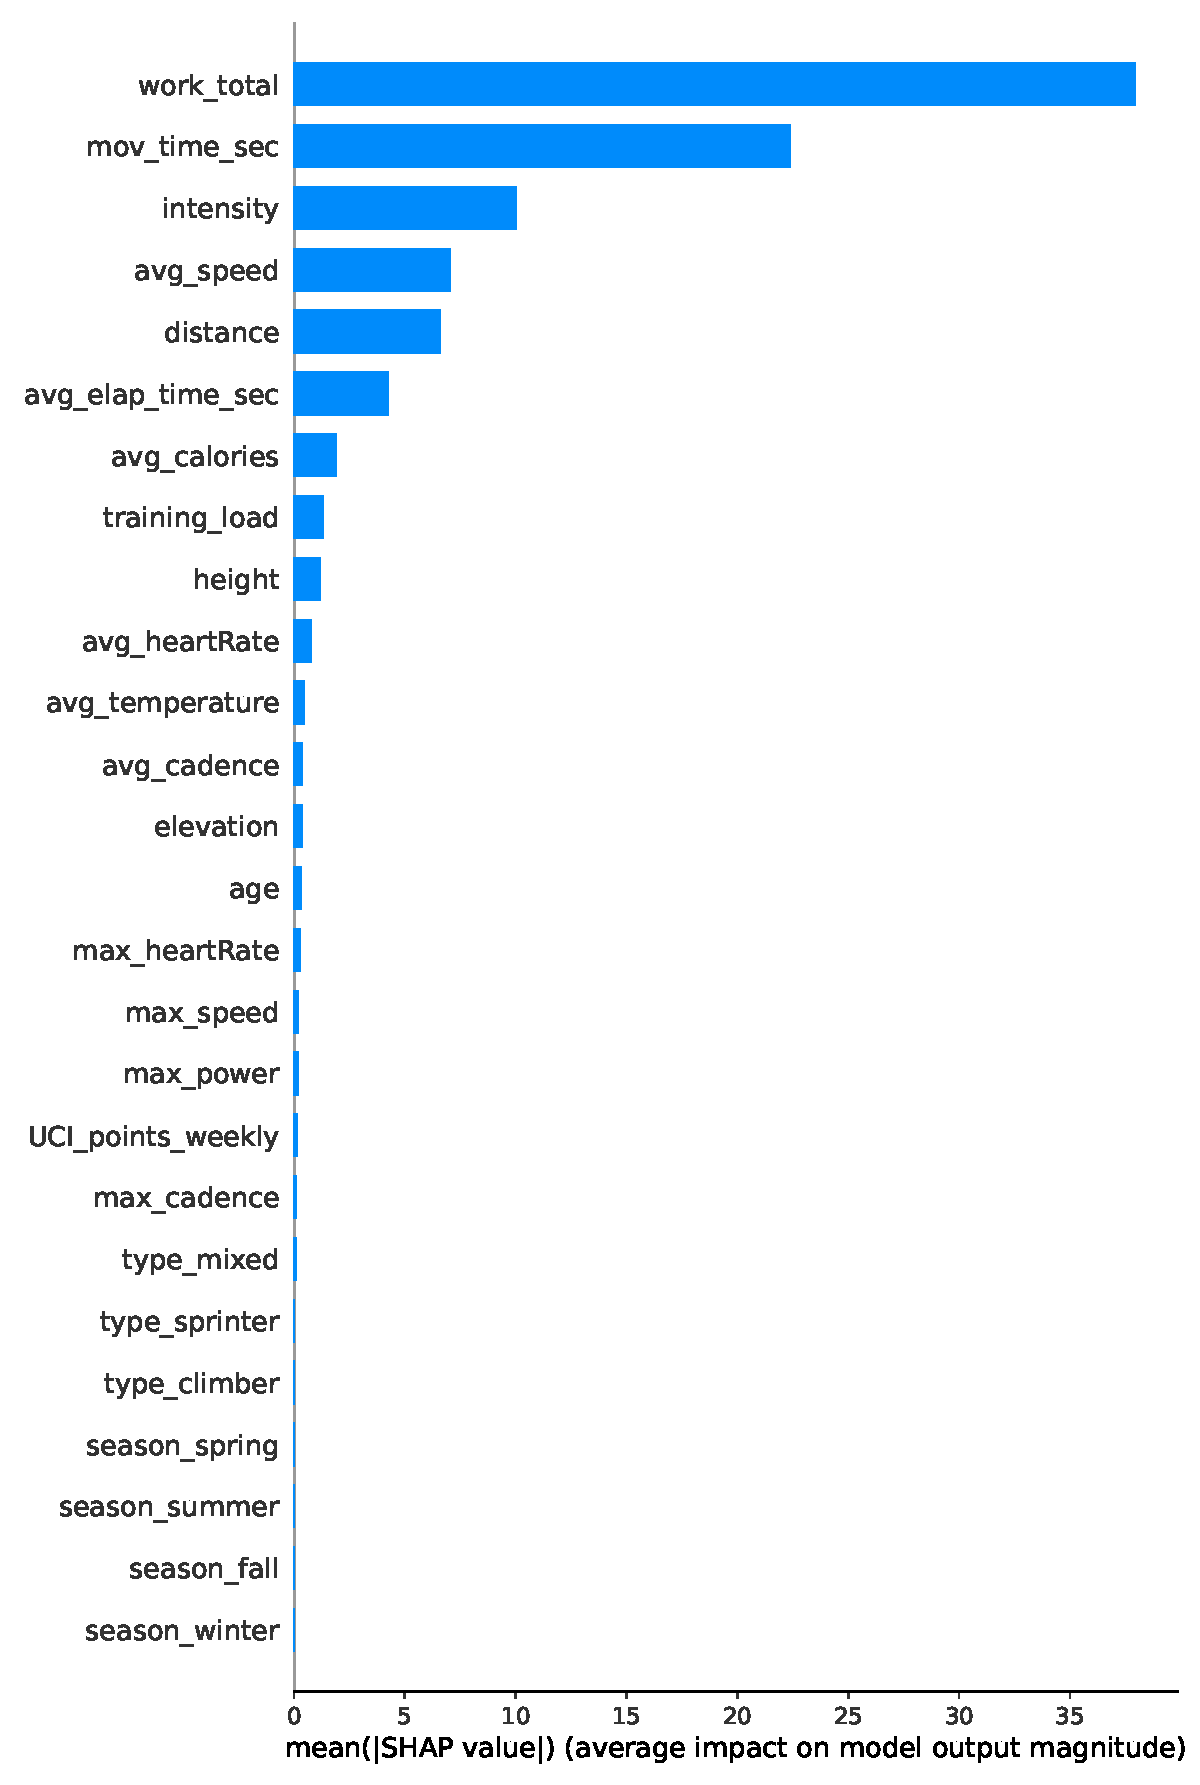
\includegraphics[width=0.8\textwidth]{./includes/shap/xgboost/summary_avg_p_bar.pdf}
    \caption{This figure shows the feature importance defined by the absolute mean Shapley values of each variable of model 3 fitted with the XGBoost algorithm. All values were calculated from the test dataset. For  }
    \label{fig:summary_avg_p_bar}
\end{figure}

Figure \ref{fig:summary_avg_p_bar} shows that the feature \(work\_total\) on (absolute) average added around 40 watts to the mean prediction value of the target variable \(avg\_power\),
while \(mov\_time\_sec\) is predicted to have the second largest impact on the prediction. If the latter feature is part of the model the average increase to the average prediction values around 20 watts. On the other hand variables with almost any contribution to the average prediction are \(UCI\_points\_weekly\) and \(max\_cadence\), \(type\) and \(season\). It seems that the weekly tournament points, the maximal cadence value of the training ride and the cycling type of an athlete are not helpful to predict the average power of a training ride of a professional athlete measured through a bicycle computer. The categorical variable \(season\) seems to have no impact at all on the model. We can therefore conclude that we do not observe any seasonal influence on the average power of a training ride. All effects describe the behavior of the model and are not necessarily causal in the real world. Furthermore we do not claim that it would not matter if a road was covered with ice, nor do we claim that snow in the winter month would have no impact on the average power of a training ride compared to a training on the same road in a summer month. A reasonable explanation of these results could be, that those professional riders, which faces seasonal influence on their training routes, might train during this time of the year in the southern hemisphere or use a static bicycle trainer at home.

\begin{figure}
\centering
\hspace{-3cm}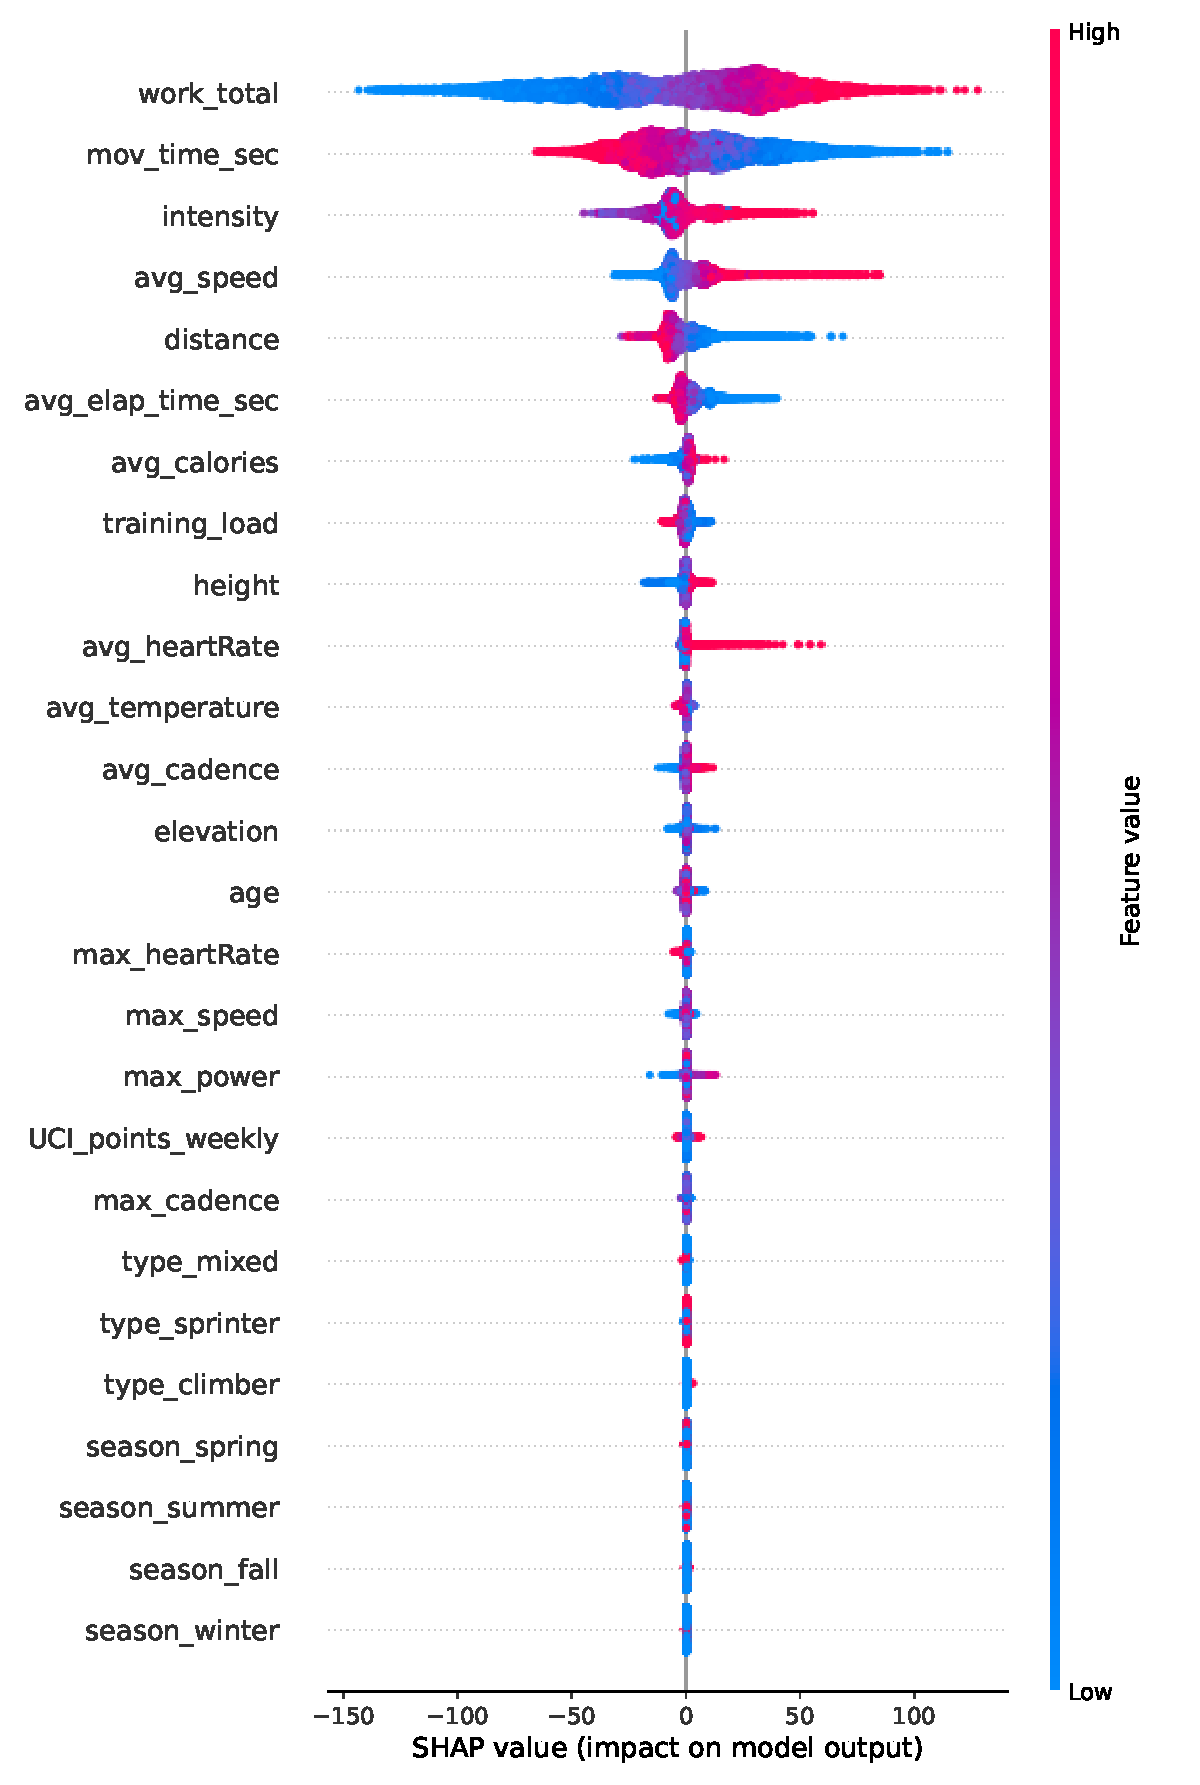
\includegraphics[width=0.8\textwidth]{./includes/shap/xgboost/summary_avg_p.pdf}
    \caption{This figure shows the summary of each variable with respect to each observation of model 3 fitted with the Catboost algorithm. All values were calculated from the test dataset. }
    \label{fig:summary_avg_p}
\end{figure}

The SHAP summary plot in figure \ref{fig:summary_avg_p} splits the feature importance bar of each feature in figure \ref{fig:summary_avg_p_bar} into their single observations and adds a heat map to reflect the feature value. More specifically, bluer dots imply a lower and redder spots a higher feature value. Grey values mark features that are categorical. For model 3, we observed that higher \(work\_total\) feature values led to a larger increase of the average prediction value of the \(avg\_power\) variable. We observed that most observations helped the model prediction by increasing or decreasing the average prediction with values between \(\mp 50\). With a slightly higher accumulation of observations around \(+50\), we expected that \(work\_total\) increased the average prediction value of the model more often than it decreases it. This helped us describe the average influence of \(work\_total\) as likely positive, which we were unable to tell just with the bar plot due to the absolute values. \(mov\_time\_sec\) feature values show an opposite effect on the average prediction of \(avg\_power\). Higher values tend to decrease the model's prediction while lower tend to increase it. This effect is in line with the intuitive judgement that a training ride shorter in time should be on average less powerful than one that requires more time. The same behavior is expected from the \(distance\) feature. A training ride that is longer in distance should decrease the average prediction of the model, as we would expect factors such as exhaustion, to reduce the overall average power that can be used during the training ride. Biological features such as \(height\) or \(age\) seem to have no large impact on the model. Taller riders show an increase of the average model prediction of the average power.Some younger professionals show a small benefit from their age in terms of a surplus of the model's prediction value, while professionals with a higher age show neither a decrease nor an increase of the model's prediction due to their age. The latter could indicate that some younger professionals might have a biological benefit while older professionals benefit from their experience gained over their career years.

\hypertarget{prediction-of-the-uci-weekly-points}{%
\subsection{Prediction of the UCI weekly points}\label{prediction-of-the-uci-weekly-points}}

\begin{figure}[!H]
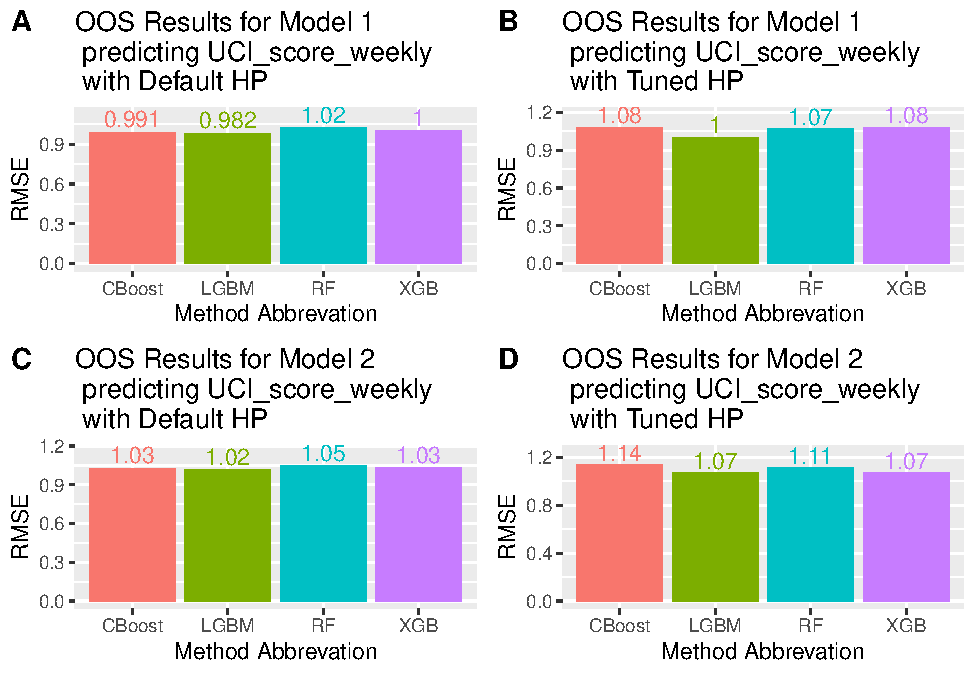
\includegraphics{Master_Thesis_files/figure-latex/RMSE-UCI-model-1-2-1} \caption{OOS results for UCI weekly points prediction with model 1 and 2}\label{fig:RMSE-UCI-model-1-2}
\end{figure}

Figure \ref{fig:RMSE-UCI-model-1-2} shows the OOS results for model 1 (A and B) and 2 (C and D) predicting the UCI weekly points. The lowest OOS RMSE value model-wise is 0.982396 given by model 1 fitted with the Lightgbm method. The worst results in terms of performance for model 1 targeting the weekly tournament points is Catboost in the tuned hyperparameter settings with an RMSE of 1.14. As already mentioned we observe a performance decrease over all methods when we compare default to tuned hyperparameter settings. A notable result is that Catboost, which was always in the top 2 method results for fitting a model, fails to repeat those results for the UCI weekly points prediction with model 2. Catboost managed to achieve the worst results in the tuned hyperparameter settings with an RMSE of 1.14. A possible explanation for the worse results from methods with tuned hyperparameter settings could be that we stopped the optimization process for all models if no RMSE improvmen was observed for 3 consecutive rounds with the Bayesian HPO. Furthermore we expect that the default settings might be near the optimal settings for this regression task and the given Strava dataset. The results are in line with our expectation from figure \ref{fig:heat-map}.

\begin{figure}[!H]
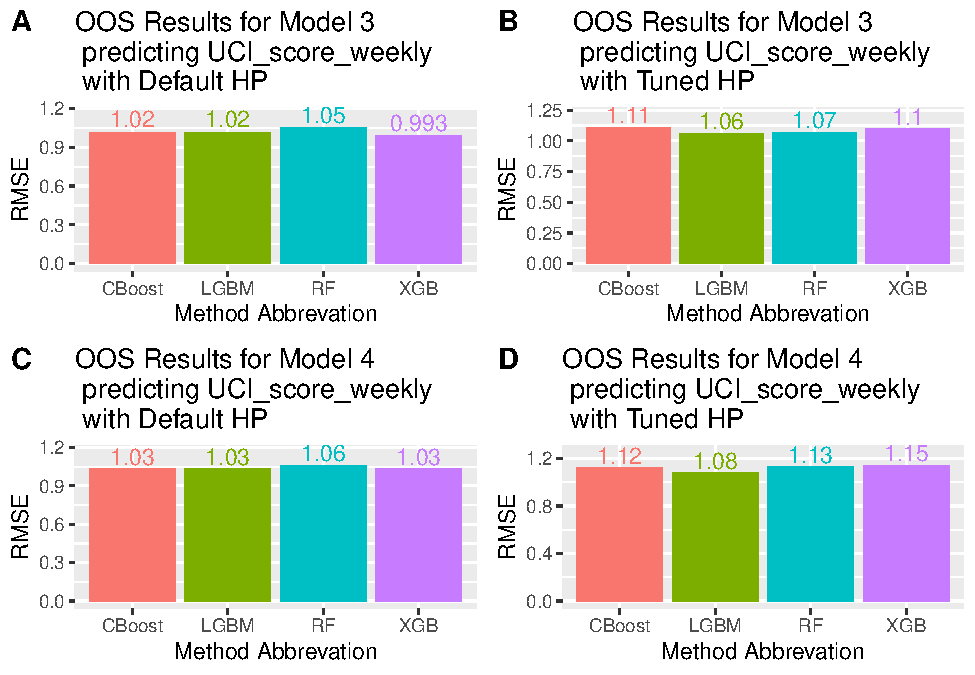
\includegraphics{Master_Thesis_files/figure-latex/RMSE-UCI-model-3-4-1} \caption{OOS results for UCI weekly points prediction with model 3 and 4}\label{fig:RMSE-UCI-model-3-4}
\end{figure}

Figure \ref{fig:RMSE-UCI-model-3-4} presents the OOS results for model 3 (A and B) and 4 (C and D) predicting the UCI weekly points. Compared to the OOS results of all other model results, model 3 managed to produce the second best performance with default hyperparameter settings. The XGBoost method accomplished an RMSE value of 0.993. For model 4 predicting the UCI weekly points, XGBoost showed the worst performance result in the OOS and tuned hyperparameter settings with an RMSE of 1.15. For the default settings Lightgbm again achieved a little lower RMSE value of 1.02 with default settings compared to all other methods.

No model-method combination managed to achieve a RMSE close to prediction of the \(avg\_power\) variable. Furthermore, we observed that for every model the OOS results of the methods with default hyperparameter settings achieved better results compared to those with tuned hyperparameter settings. These results were not useful for predicting professional rider ranks but were to some extend in line with other findings such as \textcite{Brefeld2020}. The previous authors managed to predict only 5 of the 10 ranks correctly for the Tour of Flanders in 2019. They argued that team sports might have a huge unpredictability factor, which explained the poor performance to some extend. Nevertheless, the results for the prediction of the UCI weekly points in this work are much worse then their results. We will continue with the SHAP value analysis to shed light on possible features which led to the poor model performance.

\begin{figure}
\centering
\hspace{-3cm}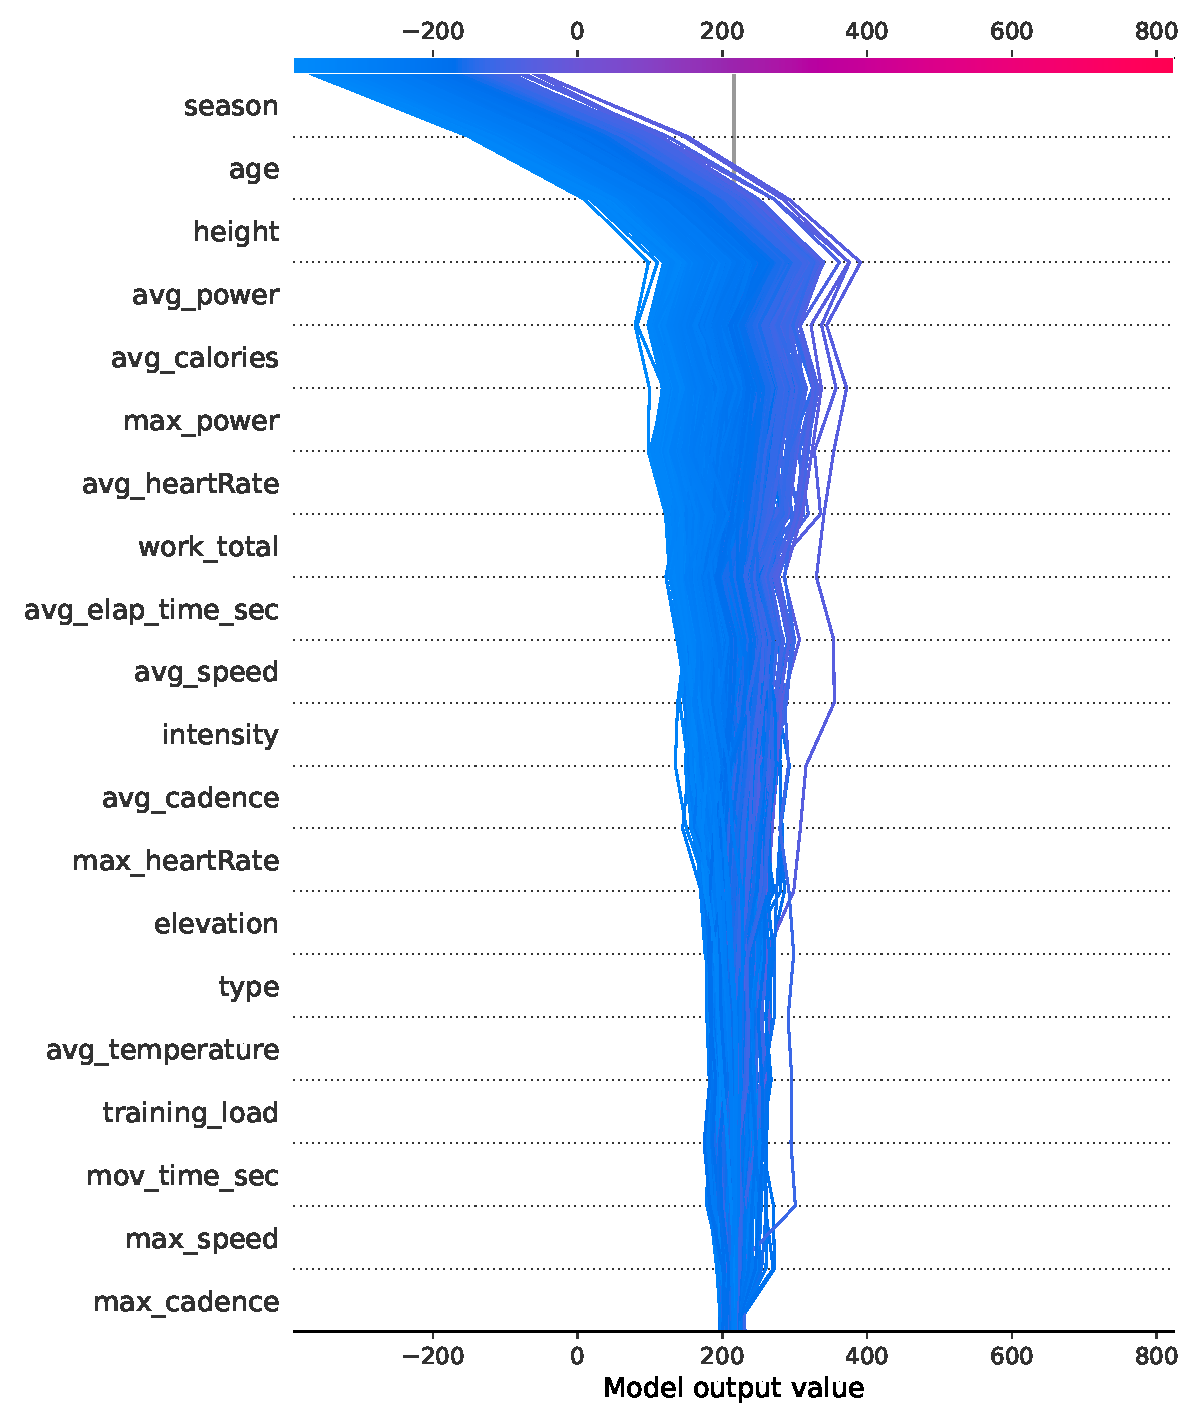
\includegraphics[width=0.8\textwidth]{./includes/shap/lightgbm/decision_UCI_points.pdf}
    \caption{This figure shows a feature decision plot of each variable  of model 1 fitted with the Lightgbm algorithm predicting the UCI weekly points. All values were calculated from the first 10.000 observations the test dataset. }
    \label{fig:decision_UCI}
\end{figure}

We will begin the SHAP analysis of model 1 which has predicted the UCI weekly points with the analyzation of figure \ref{fig:decision_UCI}. This figure shows the impact of each feature on the model prediction of the first 10.000 observations. The horizontal grey line around the value of 200 indicates the expected model prediction without any feature added. A heat map colors each observation indicating the difference from the expected model prediction. Bluer lines imply a lower and redder lines a higher outcome of the observation. Almost all values seem to be underfitted by the model. The actual range of the UCI weekly points in the first 10.000 observations of the test dataset is between {[}0;1944{]} and an average value of 224.3048. the biggest influence on the negative divergence from the mean prediction of the model are the variables \(sesaon\), \(age\) and \(height\). The variable with the forth highest influence is \(avg\_power\) which show a small positive shift towards values above the mean prediction of the model.

\begin{figure}
\centering
\hspace{-3cm}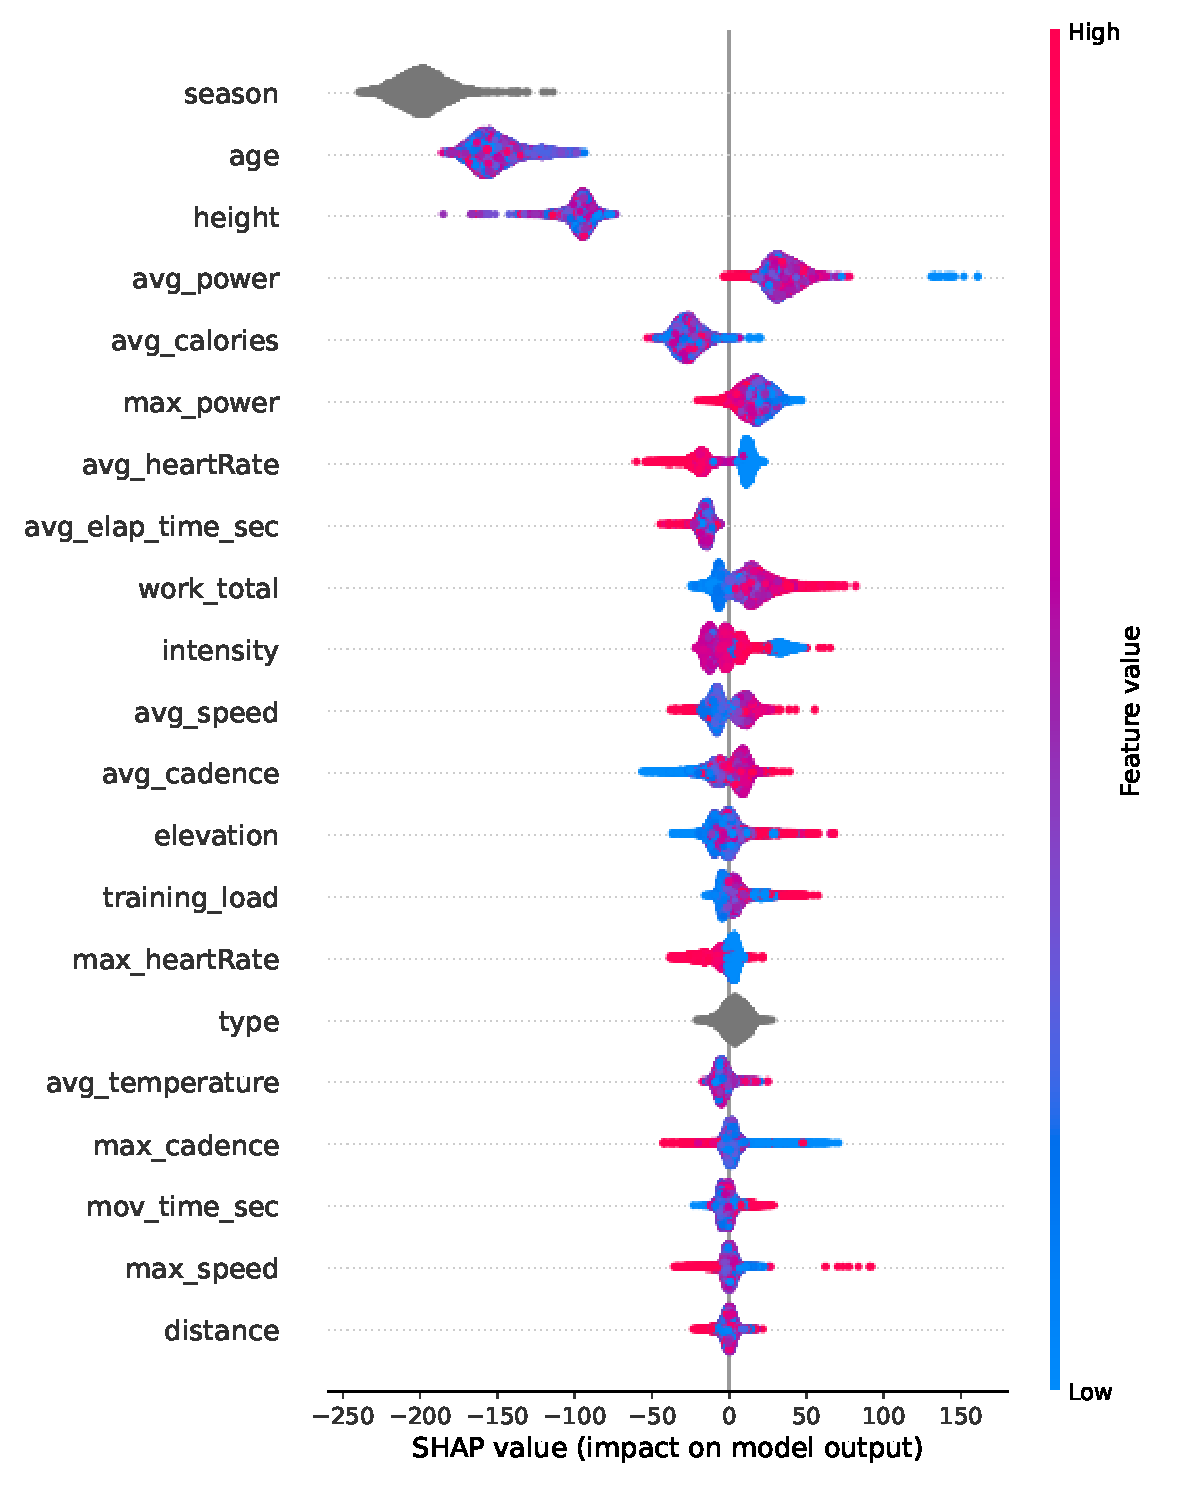
\includegraphics[width=0.8\textwidth]{./includes/shap/lightgbm/summary_UCI_points.pdf}
    \caption{This figure shows the summary of each variable with respect to each observation of model 1 fitted with the Lightgbm algorithm predicting the UCI weekly points. All values were calculated from the test dataset.}
    \label{fig:summary_UCI}
\end{figure}

Figure \ref{fig:summary_UCI} shows the summary of each feature on a heat map for the feature values of all observations. We observe no heat pattern for \(sesaon\), \(age\) or \(height\). This means that higher/lower feature values do not indicate an increase/decrease of the model predictions. As expected from figure \ref{fig:decision_UCI}, we observe that all values of those
variables show a negative impact. The difference between those three variables is the average impact indicated by clusters of the observations. For \(age\), we observe a cluster around -150, while \(height\) shows a cluster around -100. The negative impact on the average prediction of the UCI weekly points of \(age\) is therefore on average around 1.5 times higher than the impact of \(height\) on the average prediction of the UCI weekly points. A cluster with an average positive impact of around 30 is observed for the \(avg\_power\) feature. Some very low values of that feature seem to lead to an larger increase of the UCI weekly points prediction compared to the mean model output while very high values show an opposite effect. An explanation for this behavior might be that athletes who had a hard training session in the same week of some tournament might either not participate in the event or could not use their full capabilities due to their heavy exercise. Such an explanation could be supported when the feature \(avg\_heartRate\) is examined. A higher average heart rate seems to lead to a lower UCI weekly points, while the reversed effect can be expected for lower average heart rate values on the training rides.

When we removed the variables \(height\), \(season\), \(age\), \(avg\_calories\), \(avg\_elap\_time\_sec\) from the dataset and refit all models again, we saw a very small performance increase for all models. The best model is still model 1 with the default hyperparameter settings for XGBoost. The latter achieved an RMSE of 0.961 an error reduction of 0.03 compared to Lightgbm with the same model.

Figure \ref{fig:RMSE-UCI-irmi-new-avg-power-comb} presents the results for model 1 (A and B) and model 2 (B and C) while figure \ref{fig:RMSE-UCI-irmi-new-avg-power}, presents the results for model 3 (A and B) and model 4 (C and D) of the prediction of the \(UCI\_score\_weekly\) variable without the variables \(height\), \(season\), \(age\), \(avg\_calories\), \(avg\_elap\_time\_sec\). We observed a small improvement for all models with XGBoost being the method which achieves the lowest RMSE of 0.961 with model 1 and default hyperparameter settings. (A).



\begin{figure}[!H]
\includegraphics{Master_Thesis_files/figure-latex/RMSE-UCI-irmi-new-avg-power-comb-1} \caption{results for UCI weekly points prediction with model 1 and 2 without \(height\), \(season\), \(age\), \(avg\_calories\) and \(avg\_elap\_time\_sec\)}\label{fig:RMSE-UCI-irmi-new-avg-power-comb}
\end{figure}

We observed, that when we excluded those variable that had a negative impact , CatBoost and Lightgbm achieved a small \(RMSE\) decrease when they were used to fit the models 1,2 and 3 with tuned hyperparameter settings. This helps our argument that Bayesian HPO improves the predicition results for tree-based methods, even if model 1 again shows the best result when XGBoost was used with default hyperparameter settings.



\begin{figure}[!H]
\includegraphics{Master_Thesis_files/figure-latex/RMSE-UCI-irmi-new-avg-power-1} \caption{results for UCI weekly points prediction with model 3 and 3 without \(height\), \(season\), \(age\), \(avg\_calories\) and \(avg\_elap\_time\_sec\)}\label{fig:RMSE-UCI-irmi-new-avg-power}
\end{figure}

\hypertarget{bayesian-hyperparameter-tuning}{%
\subsection{Bayesian Hyperparameter Tuning}\label{bayesian-hyperparameter-tuning}}

In the case of the prediction of the average power measurements, Catboost and Lightgbm seemed to rely heavily on HPO. Random Forest and XGBoost achieved with default hyperparameter settings equally good results. XGBoost benefited more from the hyperparameter tuning in terms of RMSE reduction than Random Forest. One reason for this result might be that the Random Forest method only has 2 hyperparameter to tune in comparison to gradient boosting methods which have up to 5 hyperparameter. Furthermore those extra hyperparameter could be more valuable in terms of RMSE reduction.

Table \ref{tab:HPO_results_best_mod_short} shows the results of the Bayesian HPO and the default values of the best model with the method that achieved the lowest RMSE for both regression tasks. An overview over all methods for both best models can be found in the appendix figure \ref{tab:HPO_results_best_mod}

\begin{table}[!htbp]
\scriptsize
\centering
\captionsetup{labelsep=newline, justification=centering}
  \begin{threeparttable}
       \caption{\textit{Hyperparameter Results of the Bayesian HPO of the best model }} 
    \begin{tabular}{*{6}{l}}
        \toprule
         {Method}&  \multicolumn{1}{c}{\makecell{mtry }} & \multicolumn{1}{c}{\makecell{Minimal \\ node size }} & \multicolumn{1}{c}{\makecell{Tree Depth}} & \multicolumn{1}{c}{\makecell{ learning rate}} & \multicolumn{1}{c}{\makecell{ loss reduction}}  \\
        \midrule
        & & & \multicolumn{1}{c}{\makecell{\textbf{Model 3} \\ \textbf{ Average Power }}}& &  \\
        \midrule
        \textit{XGBoost}  &
        \multicolumn{1}{c}{\makecell{\textbf{20}\\ (all)}} & 
        \multicolumn{1}{c}{\makecell{\textbf{40} \\ (1)}} & 
        \multicolumn{1}{c}{\makecell{\textbf{14}\\ (6)}}  &
        \multicolumn{1}{c}{\makecell{\textbf{0.0729534}\\ (0.3)}}&
        \multicolumn{1}{c}{\makecell{\boldmath{\ensuremath{4.7306132\times 10^{-4}}} \\ (0)}}
\\
        \midrule
        & & & \multicolumn{1}{c}{\makecell{\textbf{Model 1} \\ \textbf{UCI weekly points }}}&  & \\ 
        \midrule
        \textit{XGBoost}  &
        \multicolumn{1}{c}{\makecell{9 \\ \textbf{(all)}}} & 
        \multicolumn{1}{c}{\makecell{3 \\\textbf{(1)}}} & 
        \multicolumn{1}{c}{\makecell{14 \\\textbf{(6)}}}  &
        \multicolumn{1}{c}{\makecell{0.020941 \\ \textbf{(0.03)}}}&
        \multicolumn{1}{c}{\makecell{\ensuremath{5.0319939\times 10^{-5}} \\ \textbf{(0)}}}
\\
        \bottomrule
     \end{tabular}
    \begin{tablenotes}[flushleft]
      \small
      \item \textit{Note.} Values in square brackets indicate the default hyperparameter settings. Bold numbers indicate the hyperparameter settings of the method which achieved the lowest RMSE for the best model. '-' indicates that this hyperparameter is not available for tuning. The stop condition of the HPO was 3 consecutive rounds without an RMSE improvement of the model. All methods generated 1000 trees. *x indicates the number of variables of the train dataset. 
    \end{tablenotes}
      \label{tab:HPO_results_best_mod_short}
  \end{threeparttable}
\end{table}

We detected that for the Strava dataset a combination of 20 features with at least 40 observations in a node to continue splitting, a maximum tree depth of 14, a learning rate of 0.0729534 and almost 0 but still positive loss reduction of \ensuremath{4.7306132\times 10^{-4}} led to the best OOS RMSE results of model 3 predicting the average power of the training sessions. For the prediction of the UCI weekly points, we observed that fitting model 1 with XGBoost using the default hyperparameter settings described in table \ref{tab:HPO_results_best_mod} section Model 1 UCI weekly points led to the best OOS RMSE results.

\hypertarget{discussion}{%
\section{\texorpdfstring{Discussion \label{sec:discussion}}{Discussion }}\label{discussion}}

There is a high correlation between \(avg\_power\) and \(work\_load\) which is likely due to the same information, power expressed in watts, was used to calculate both variables by the bicycle computer. This might have lead to some form of target leakage in the sense that some information about the average power is already contained in the \(work\_load\). We considered this and used the model with the highest prediction power in terms of the lowest OOS RMSE value to predict \(avg\_power\) again without \(work\_load\) in the Strava dataset.

\begin{table}[!htbp]
\small
\begin{center}
\captionsetup{labelsep=newline, justification=centering}
  \begin{threeparttable}
       \caption{\textit{OOS RMSE results for all models predicting the average power without $work\_load$ }} 
    \begin{tabular}{*{5}{l}}
        \toprule
         {Method}&  \multicolumn{1}{c}{\makecell{Model 1 }} & \multicolumn{1}{c}{\makecell{Model 2 }} & \multicolumn{1}{c}{\makecell{Model 3  }} & \multicolumn{1}{c}{\makecell{ Model 4}}  \\
        \midrule
        & & \multicolumn{1}{c}{\makecell{\textbf{ Default Hyperparameters }}}& & \\
        \midrule
        \textit{RF}   & \multicolumn{1}{c}{\makecell{0.434}} &
        \multicolumn{1}{c}{\makecell{0.412}} & 
        \multicolumn{1}{c}{\makecell{0.388}}  &
        \multicolumn{1}{c}{\makecell{0.404}}
\\
        \textit{LGBM}  & \multicolumn{1}{c}{\makecell{0.866}} &
        \multicolumn{1}{c}{\makecell{0.851}} & 
        \multicolumn{1}{c}{\makecell{0.866}}  &
        \multicolumn{1}{c}{\makecell{0.861}}
\\
        \textit{XGBoost}  & \multicolumn{1}{c}{\makecell{0.478}} &
        \multicolumn{1}{c}{\makecell{0.459}} & 
        \multicolumn{1}{c}{\makecell{0.432}}  &
        \multicolumn{1}{c}{\makecell{0.449}}
\\
        \textit{Catboost}  & \multicolumn{1}{c}{\makecell{0.996}} &
        \multicolumn{1}{c}{\makecell{0.991}} & 
        \multicolumn{1}{c}{\makecell{1.001}}  &
        \multicolumn{1}{c}{\makecell{1.003}}
\\
        \midrule
        & & \multicolumn{1}{c}{\makecell{\textbf{Tuned Hyperparameters}}}& & \\ 
        \midrule
        \textit{RF}   & \multicolumn{1}{c}{\makecell{0.42}} &
        \multicolumn{1}{c}{\makecell{0.394}} & 
        \multicolumn{1}{c}{\makecell{0.386}}  &
        \multicolumn{1}{c}{\makecell{0.392}}
\\
        \textit{LGBM} & \multicolumn{1}{c}{\makecell{0.335}} &
        \multicolumn{1}{c}{\makecell{0.319}} & 
        \multicolumn{1}{c}{\makecell{0.293}}  &
        \multicolumn{1}{c}{\makecell{0.32}}
\\
        \textit{XGBoost}  & \multicolumn{1}{c}{\makecell{0.35}} &
        \multicolumn{1}{c}{\textbf{\makecell{0.316}}} & 
        \multicolumn{1}{c}{\makecell{\textbf{0.297}}}  &
        \multicolumn{1}{c}{\textbf{\makecell{0.305}}}
\\
        \textit{Catboost}  & \multicolumn{1}{c}{\textbf{\makecell{0.33}}} &
        \multicolumn{1}{c}{\makecell{0.344}} & 
        \multicolumn{1}{c}{\makecell{0.321}}  &
        \multicolumn{1}{c}{\makecell{0.309}}
\\
        \bottomrule
     \end{tabular}
    \begin{tablenotes}[flushleft]
      \small
      \item \textit{Note.} Bold numbers indicate the lowest RMSE for each model. Hyperparameter tuning was performed with Bayesian HPO for all methods.
    \end{tablenotes}
      \label{tab:OOS_results_avg_pow_work_load}
  \end{threeparttable}
  \end{center}
\end{table}

The results are presented in table \ref{tab:OOS_results_avg_pow_work_load}. We observe a comparable pattern to the OOS results of the models containing the variable \(work\_load\). The RMSE is always lower when the method used tuned hyperparameter settings compared to the default settings for all models. In contrast we observe that either Catboost or XGBoost are the best performing methods for models 1 and 2,3,4, respectively. With model 3 now achieving the lowest RMSE of 0.297 which equals to an \(R^2\) metric value of 0.908. So that even without the \(work\_load\) variable we can explain more than 90\% of the variance of the predicted average power.

\textcite{Amoukou2021} claimed that SHAP values for tree ensembles might not be exact especially if the model had some one-hot encoded categorical variables. They argued that this happens due to the break of a fundamental property of SHAP values, namely the symmetry property or equal treatment of equals.

The Strava dataset had two categorical variables namely \(season\) and \(type\). \(Cramesr's V\) is a correlation measure between two nominal variables.
\begin{equation}
\text {Cramer's } V=\sqrt{\left(X^{2} / n\right) / \min (c-1, r-1)}
\end{equation}
where \(X^2\) defines the chi-square statistic, \(n\) the number of observations, \(r\) the number of rows and \(c\) the number of columns. The range is between 0 and 1. The \(Cramesr's V\) between \(season\) and \(type\) is 0.1247. Therefore we observe a low but positive correlation between these two variables. A simple example shows how this leads to biased SHAP values. Consider \(Y = 100 \times X_1 + 100 \times X_1\) be a simple model. With \(X_1\) and \(X_2\) were both Bernoulli variables of parameter \(p_1=p_2=0.5\) and 1000 observations.

\begin{table}[!htbp]
\small
\begin{center}
\captionsetup{labelsep=newline, justification=centering}
  \begin{threeparttable}
       \caption{\textit{Repartition of $X_1$ and $X_2$ }} 
    \begin{tabular}{*{3}{l}}
 \toprule
     \multicolumn{1}{c}{\makecell{\textbf{ Observations  }}}   &\multicolumn{1}{c}{\makecell{\textbf{ $X_1$ }}} & \multicolumn{1}{c}{\makecell{\textbf{ $X_2$ }}} \\
     \midrule
      \multicolumn{1}{c}{\makecell{\textbf{ 400  }}}   &\multicolumn{1}{c}{\makecell{\textbf{ 0 }}} & \multicolumn{1}{c}{\makecell{\textbf{ 0 }}} \\
      \multicolumn{1}{c}{\makecell{\textbf{ 100  }}}   &\multicolumn{1}{c}{\makecell{\textbf{ 1 }}} & \multicolumn{1}{c}{\makecell{\textbf{ 0 }}} \\ 
      \multicolumn{1}{c}{\makecell{\textbf{ 100  }}}   &\multicolumn{1}{c}{\makecell{\textbf{ 0 }}} & \multicolumn{1}{c}{\makecell{\textbf{ 1 }}} \\
      \multicolumn{1}{c}{\makecell{\textbf{ 400  }}}   &\multicolumn{1}{c}{\makecell{\textbf{ 1 }}} & \multicolumn{1}{c}{\makecell{\textbf{ 1 }}} \\ 
      \bottomrule
      \end{tabular}
        \label{tab:repartition}
       \end{threeparttable}
  \end{center}
\end{table}

Table \ref{tab:repartition} represents the repartition of the the latter variables :
Since this is symmetrical in \(X_1\) and \(X_2\) we should observe equal SHAP values without considering the correlation between these two variables.

\begin{figure}
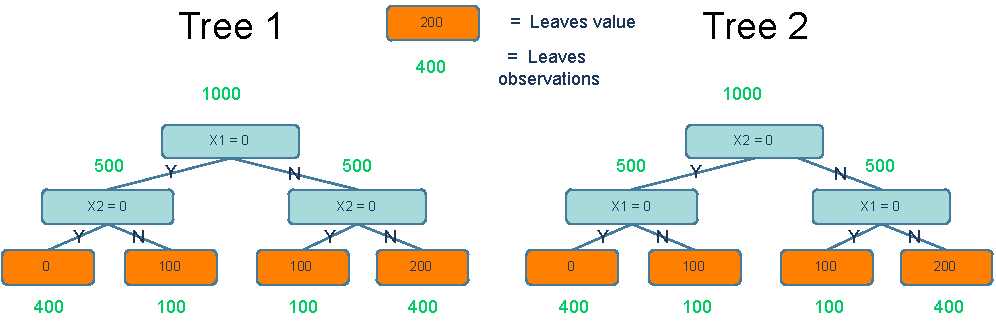
\includegraphics[height = 20cm, width = \linewidth]{./includes/SHAP_bias.pdf}
    \caption{Diagram of the two tree versions of the simple model $Y = 100 \times X_1 + 100 \times X_1$. The values with a green number representing the subset of the dataset at a given split while the numbers in the leave nodes representing the value of the leaves.}
    \label{fig:tree_shap_bias}
\end{figure}

Following \textcite{Amoukou2021}, table \ref{tab:SHAP_bias} shows the calculation of the SHAPE values of the simple model given that \(X_1\) and \(X_2\) share a positive correlation. The latter is represented by two trees of depth 2, each tree represented one version of the model depending on the order or \(X_1\) and \(X_2\). A visualization of of the aforementioned tree representation of the bias is given in figure \ref{fig:tree_shap_bias}. We also calculated the bias of this example. Table \ref{tab:SHAP_bias} in the appendix shows that the SHAP values are not symmetric. We follow \textcite{Amoukou2021} and assume that in general SHAP values for tree ensembles are biased if two categorical variables in a dataset share a positive correlation and were used at least once as a splitting criterion. Therefore we assume that the SHAP values for the prediction of average power and the weekly UCI score were biased as well. \textcite{Amoukou2021} presented a solution to this problem by adjusting the highlighted weights in table \ref{tab:SHAP_bias}. To account for the correlation for tree 1, one needs to adjust the total observations with respect to \(X_2=1\) from 1000 to 500, adjust the observations of the subset for \(X_1=0\) with respect to \(X_2=1\) from 500 to 100 and adjust the observations of the subset for \(X_1 =1\) with respect to \(X_2 = 1\) from 500 to 400. In return, SHAP values for tree methods will be independent from the correlation of two categorical variables and thereby exact as stated by \textcite{Lundberg2017}. We recognized the latter findings but were not able to implement them in this work as they have only recently appeared. The author would like to stress that this bias might be limited to those tree ensemble methods which require encoding techniques that extend the feature matrix such as one-hot-encoding. If we understand \textcite{Amoukou2021} this bias should not concern results obtained from the Catboost models since Catboost uses target encoding for categorical variables which does not extend the feature matrix. Furthermore, the symmetric tree-building strategy used by Catboost leads to tree paths that are always symmetric.

Furthermore we would like to stress that a higher stopping criterion than 3 consecutive rounds without RMSE improvement for the Bayesian HPO algorithm could lead to better results for the UCI weekly points prediction. \textcite{Hvarfner2022} showed Bayesian HPO can be further improved in terms of time-to-accuracy if one uses a prior belief about a location where an optimum with some hyperparameter settings occurs. The prior belief will be integrated through an adjustment of the acquisition function. Since this prior belief requires some expert's opinion about the dataset and the machine-learning algorithm we suggest, that a possible prior could be generated from literature of comparable machine-learning tasks. If such literature exists one could use the average of each hyperparameter of the given papers as their expert's prior. Another suggestions might be to use the hyperparameter of the most recent paper featuring a comparable machine-learning tasks and the same methods.

\hypertarget{conclusion}{%
\section{Conclusion}\label{conclusion}}

In this thesis we showed that we can successfully predict the average power of training sessions of professional road cyclists with a precision up to 0.978 for the \(R^2\) metric and an RMSE of 0.1496695 including all variables of the Strava dataset. When we excluded \(work\_total\), which was probably calculated using measurements as for the calculation of the average power measurement from the Strava dataset and therefore might have led to biased results, we achieved a \(R^2\) metric in the OOS testing of 0.908 and an RMSE of 0.305. Furthermore we showed that neither a specific season nor a specific cycling type, \(sprinter\),\(climber\) or \(mixed\), helps to improve the average power of a professional road cyclists. Model 3 featured imputed values, using the IRMI algorithm, for the variables of the average temperature and the average calories during the training session. When \(work\_total\) was removed from the feature list a drop of almost 8 percentage points of the \(R^2\) value was observed. Future research questions could involve the possibility to replace \(work\_total\) with an instrumental variable uncorrelated to the average power measure. This helped the argument that less conservative solutions to handle missing values, e.g.~imputing strategies, can be a promising alternative to improve a models prediction quality. We failed to reproduce results with a comparable high performance, predicting the UCI weekly points. The lowest RMSE for the OOS scenario we were able to achieve was 0.982396 which is equal to a \(R^2\) value of 0.982396. SHAP Values helped in both cases to improve the explainability of the models. For the average power prediction the figures of the SHAP values revealed that the variable \(work\_total\) and \(move\_time\_sec\) had the biggest impact on the models prediction. For the prediction of the UCI weekly points,figures of the SHAP values of the model 1 fitted with the Lightgbm method and default hyperparameter settings gave us the insight that the variables \(seaon\), \(age\), \(height\), \(avg\_elap\_time\_sec\) showed an overall negative impact. The feature decision plot of the SHAP values indicated that the predictions were much lower than the actual values. This led us to the idea to extract those variables and refit the model with only variables with a possible positive impact on the model. Thereby we achieved an RMSE value of 0.9612489 which equals an \(R^2\) of 0.0685645 an improvement of more than 2 percentage points compared to the models that contained the aforementioned variables with negative impact. The tree SHAP algorithm, as described by \textcite{Lundberg2017}, seems to be biased if a non-zero correlation between one-hot-encoded variables exists in a dataset. Following \textcite{Amoukou2021} a possible solution to this bias is described but was not implemented. A comparison between the biased and possible unbiased SHAP values of the best models and methods combination the both regression tasks in this thesis could be a possibility for future research. Especially to clarify if the Catboost algorithm with his own target encoding of nominal variable suffers from the same kind of bias as well. Furthermore we have shown that tree-based ensemble methods achieve better prediction results for the average power with the Strava dataset if their hyperparameter were optimized instead of using the default hyperparameter settings. We argue, that using Bayesian HPO for the latter optimization produced on average better results in the same computational time compared to other HPO methods, since a continuous evaluation of the results helped to chose hyperparameter that have a higher chance of coming close to the optimal settings for the regression task. Improvement of this procedure was discussed via the use of an experts belief as a prior. Future research could decrease their effort in terms of computational time to optimize their preferred models.

\printbibliography

\pagebreak

\appendix

\hypertarget{appendix}{%
\section{\texorpdfstring{Appendix \label{sec:appendix}}{Appendix }}\label{appendix}}

\begin{table}[!htbp]
\scriptsize
\centering
\captionsetup{labelsep=newline, justification=centering}
  \begin{threeparttable}
       \caption{\textit{Hyperparameter results of the Bayesian HPO of the best model }} 
    \begin{tabular}{*{6}{l}}
        \toprule
         {Method}&  \multicolumn{1}{c}{\makecell{mtry }} & \multicolumn{1}{c}{\makecell{Minimal \\ node size }} & \multicolumn{1}{c}{\makecell{Tree Depth}} & \multicolumn{1}{c}{\makecell{ learning rate}} & \multicolumn{1}{c}{\makecell{ loss reduction}}  \\
        \midrule
        & & & \multicolumn{1}{c}{\makecell{\textbf{Model 3} \\ \textbf{ Average Power }}}& &  \\
        \midrule
        \textit{RF}   & 
        \multicolumn{1}{c}{\makecell{11   \\($\left\lfloor \sqrt{x} \right\rfloor$*)}} &
        \multicolumn{1}{c}{\makecell{-}}  &
        \multicolumn{1}{c}{\makecell{-}} &
        \multicolumn{1}{c}{\makecell{-}} 
        
\\
        \textit{LGBM}&
        \multicolumn{1}{c}{\makecell{15  \\(all)}} & 
        \multicolumn{1}{c}{\makecell{15 \\ (20)}} & 
        \multicolumn{1}{c}{\makecell{5\\ (no limit)}}  &
        \multicolumn{1}{c}{\makecell{0.0473691 \\ (0.1)}}&
        \multicolumn{1}{c}{\makecell{0.1186154 \\ (0)}}
        
\\
        \textit{XGBoost}  &
        \multicolumn{1}{c}{\makecell{\textbf{20}\\ (all)}} & 
        \multicolumn{1}{c}{\makecell{\textbf{40} \\ (1)}} & 
        \multicolumn{1}{c}{\makecell{\textbf{14}\\ (6)}}  &
        \multicolumn{1}{c}{\makecell{\textbf{0.0729534}\\ (0.3)}}&
        \multicolumn{1}{c}{\makecell{\boldmath{\ensuremath{4.7306132\times 10^{-4}}} \\ (0)}}
        

\\
        \textit{Catboost}  &
        \multicolumn{1}{c}{\makecell{17\\ (all)}} & 
        \multicolumn{1}{c}{\makecell{32 \\(1)}} & 
        \multicolumn{1}{c}{\makecell{14 \\(6)}}  &
        \multicolumn{1}{c}{\makecell{0.0321339 \\(0.03)}}& 
        \multicolumn{1}{c}{\makecell{-}}
        
\\
        \midrule
        & & & \multicolumn{1}{c}{\makecell{\textbf{Model 1} \\ \textbf{UCI weekly points }}}&  & \\ 
        \midrule
        \textit{RF}   &
        \multicolumn{1}{c}{\makecell{11 \\ ($\left\lfloor \sqrt{x} \right\rfloor$*) }} &
        \multicolumn{1}{c}{\makecell{2\\ (5)}} & 
        \multicolumn{1}{c}{\makecell{-}}  &
        \multicolumn{1}{c}{\makecell{-}} &
        \multicolumn{1}{c}{\makecell{-}} 
        
\\
        \textit{LGBM}&
        \multicolumn{1}{c}{\makecell{18\\ (all)}} & 
        \multicolumn{1}{c}{\makecell{11\\ (20)}} & 
        \multicolumn{1}{c}{\makecell{15 \\ (no limit)}}  &
        \multicolumn{1}{c}{\makecell{0.0190382 \\ (0.1)}}&
        \multicolumn{1}{c}{\makecell{\ensuremath{1.3131895\times 10^{-9}} \\ (0)}}
        
\\
        \textit{XGBoost}  &
        \multicolumn{1}{c}{\makecell{9 \\ \textbf{(all)}}} & 
        \multicolumn{1}{c}{\makecell{3 \\ \textbf{(1)}}} & 
        \multicolumn{1}{c}{\makecell{14 \\ \textbf{(6)}}}  &
        \multicolumn{1}{c}{\makecell{0.020941 \\ \textbf{(0.03)}}}&
        \multicolumn{1}{c}{\makecell{\ensuremath{5.0319939\times 10^{-5}} \\ \textbf{(0)}}}
        

\\
        \textit{Catboost}  &
        \multicolumn{1}{c}{\makecell{19 \\ (all)}} & 
        \multicolumn{1}{c}{\makecell{5 \\ (1)}} & 
        \multicolumn{1}{c}{\makecell{13 \\ (6)}}  &
        \multicolumn{1}{c}{\makecell{0.0861325 \\ (0.03)}}&
        \multicolumn{1}{c}{\makecell{-}} 
        
\\
        \bottomrule
     \end{tabular}
    \begin{tablenotes}[flushleft]
      \small
      \item \textit{Note.} Values in square brackets indicate the default hyperparameter settings. Bold numbers indicate the hyperparameter settings of the method which achieved the lowest RMSE for the best model. '-' indicates that this hyperparameter is not available for tuning. The stop condition of the HPO was 3 consecutive rounds without an RMSE improvement of the model. All methods generated 1000 trees. *x indicates the number of variables of the train dataset. 
    \end{tablenotes}
      \label{tab:HPO_results_best_mod}
  \end{threeparttable}
\end{table}

\newcommand{\hlfancy}[2]{\sethlcolor{#1}\hl{#2}}

\begin{table}[!htbp]
\centering
\scriptsize
\captionsetup{labelsep=newline, justification=centering}
  \begin{threeparttable}
       \caption{\textit{SHAP Value calculation with bias }} 
    \begin{tabular}{*{5}{l}}
        \toprule
        & & \multicolumn{1}{c}{\makecell{\textbf{ Tree 1 }}}& & \\
        \midrule
        \multicolumn{1}{c}{\makecell{Feature \\ subset $(S)$}}&  \multicolumn{1}{c}{\makecell{$f_x(S)$}} & \multicolumn{1}{c}{\makecell{$f_{x}(S \cup\{X_1\})$}} & \multicolumn{1}{c}{\makecell{$f_{x}(S \cup\{X_1\}$\\$ - f_x(S))$ }} & \multicolumn{1}{c}{\makecell{ $|S| !(M-|S|-1) !$}}  \\
        \midrule
        \textit{$\emptyset$}   &
        \multicolumn{1}{c}{\makecell{$100$}} &
        \multicolumn{1}{c}{\makecell{$\dfrac{100}{500} * 100 + \dfrac{400}{500} * 200 $\\$= 180$}} & 
        \multicolumn{1}{c}{\makecell{$80$}}  &
        \multicolumn{1}{c}{\makecell{$0.5$}} 
\\
        \midrule
        \textit{\{$X_2$\}}   &
        \multicolumn{1}{c}{\makecell{\sethlcolor{yellow}\hl{$\dfrac{500}{1000}$}$ * 100+ $\sethlcolor{yellow}\hl{$\dfrac{500}{1000}$}$ * 200 $\\$= 150$}} &
        \multicolumn{1}{c}{\makecell{$200$}} & 
        \multicolumn{1}{c}{\makecell{$50$}}  &
        \multicolumn{1}{c}{\makecell{$0.5$}} 
\\
\midrule 
\midrule
&&&  \multicolumn{1}{c}{\makecell{SHAP value of $X_1$}} &  \multicolumn{1}{c}{\makecell{$90$}} \\
        \cmidrule{4-5}
       \multicolumn{1}{c}{\makecell{Feature \\ subset $(S)$}}&  \multicolumn{1}{c}{\makecell{$f_x(S)$}} & \multicolumn{1}{c}{\makecell{$f_{x}(S \cup\{X_2\})$}} & \multicolumn{1}{c}{\makecell{$f_{x}(S \cup\{X_2\} $\\$ - f_x(S))$ }} & \multicolumn{1}{c}{\makecell{ $|S| !(M-|S|-1) !$}}  \\
        \midrule
        \textit{$\emptyset$}   &
        \multicolumn{1}{c}{\makecell{$100$}} &
        \multicolumn{1}{c}{\makecell{\sethlcolor{yellow}\hl{$\dfrac{500}{1000}$}$ * 100 + $\sethlcolor{yellow}\hl{$\dfrac{500}{1000}$}$ * 200 $\\$= 150$}} & 
        \multicolumn{1}{c}{\makecell{$50$}}  &
        \multicolumn{1}{c}{\makecell{$0.5$}} 
\\
        \midrule
        \textit{\{$X_1$\}}   &
        \multicolumn{1}{c}{\makecell{$\dfrac{100}{500} * 100 + \dfrac{400}{500} * 200 $\\$= 180$}} &
        \multicolumn{1}{c}{\makecell{$200$}} & 
        \multicolumn{1}{c}{\makecell{$20$}}  &
        \multicolumn{1}{c}{\makecell{$0.5$}} 
\\
\midrule  
\midrule
&&&  \multicolumn{1}{c}{\makecell{SHAP value of $X_2$}} &  \multicolumn{1}{c}{\makecell{$35$}} \\
  \cmidrule{4-5}
        & & \multicolumn{1}{c}{\makecell{\textbf{ Tree 2 }}}& & \\
        \midrule
        \multicolumn{1}{c}{\makecell{Feature \\ subset $(S)$}}&  \multicolumn{1}{c}{\makecell{$f_x(S)$}} & \multicolumn{1}{c}{\makecell{$f_{x}(S \cup\{X_1\})$}} & \multicolumn{1}{c}{\makecell{$f_{x}(S \cup\{X_1\} $\\$ - f_x(S))$}} & \multicolumn{1}{c}{\makecell{ $|S| !(M-|S|-1) !$}}  \\
        \midrule
            \textit{$\emptyset$}   &
        \multicolumn{1}{c}{\makecell{$100$}} &
        \multicolumn{1}{c}{\makecell{\sethlcolor{yellow}\hl{$\dfrac{500}{1000}$}$ * 100 + $\sethlcolor{yellow}\hl{$\dfrac{500}{1000}$}$ * 200 $\\$= 150$}} & 
        \multicolumn{1}{c}{\makecell{$50$}}  &
        \multicolumn{1}{c}{\makecell{$0.5$}} 
\\
        \midrule
        \textit{\{$X_2$\}}   &
        \multicolumn{1}{c}{\makecell{$\dfrac{100}{500} * 100 + \dfrac{400}{500} * 200 $\\$= 180$}} &
        \multicolumn{1}{c}{\makecell{$200$}} & 
        \multicolumn{1}{c}{\makecell{$20$}}  &
        \multicolumn{1}{c}{\makecell{$0.5$}} 
\\          
\midrule  
\midrule
&&&  \multicolumn{1}{c}{\makecell{SHAP value of $X_1$}} &  \multicolumn{1}{c}{\makecell{$35$}} \\
        \cmidrule{4-5}
       \multicolumn{1}{c}{\makecell{Feature \\ subset $(S)$}}&  \multicolumn{1}{c}{\makecell{$f_x(S)$}} & \multicolumn{1}{c}{\makecell{$f_{x}(S \cup\{X_2\})$}} & \multicolumn{1}{c}{\makecell{$f_{x}(S \cup\{X_2\} $\\$ - f_x(S))$}} &
       \multicolumn{1}{c}{\makecell{ $|S| !(M-|S|-1) !$}}  \\
        \midrule
\textit{$\emptyset$}   &
        \multicolumn{1}{c}{\makecell{$100$}} &
        \multicolumn{1}{c}{\makecell{$\dfrac{100}{500} * 100 + \dfrac{400}{500} * 200 $\\$ = 180$}} & 
        \multicolumn{1}{c}{\makecell{$80$}}  &
        \multicolumn{1}{c}{\makecell{$0.5$}} 
\\
        \midrule
        \textit{\{$X_1$\}}   &
         \multicolumn{1}{c}{\makecell{\sethlcolor{yellow}\hl{$\dfrac{500}{1000}$}$ * 100 + $\sethlcolor{yellow}\hl{$\dfrac{500}{1000}$}$ * 200 $\\$= 150$}} &
        \multicolumn{1}{c}{\makecell{$200$}} & 
        \multicolumn{1}{c}{\makecell{$50$}}  &
        \multicolumn{1}{c}{\makecell{$0.5$}} 
\\
\midrule
\midrule
&&&  \multicolumn{1}{c}{\makecell{SHAP value of $X_2$}} &
\multicolumn{1}{c}{\makecell{$90$}} \\
\cmidrule{4-5}
\bottomrule
     \end{tabular}
    \begin{tablenotes}[flushleft]
      \small
      \item \textit{Note.} SHAP values were calculated using equation 2 of \textcite{Lundberg2017}. In case of $|S|=\emptyset$ the author considered $0! = 1$. Highlighted parts of the calculation are weights which cause the bias of the SHAP values, argued by \textcite{Amoukou2021}. 
    \end{tablenotes}
    \label{tab:SHAP_bias}
  \end{threeparttable}
\end{table}

\begin{sidewaysfigure}[ht]
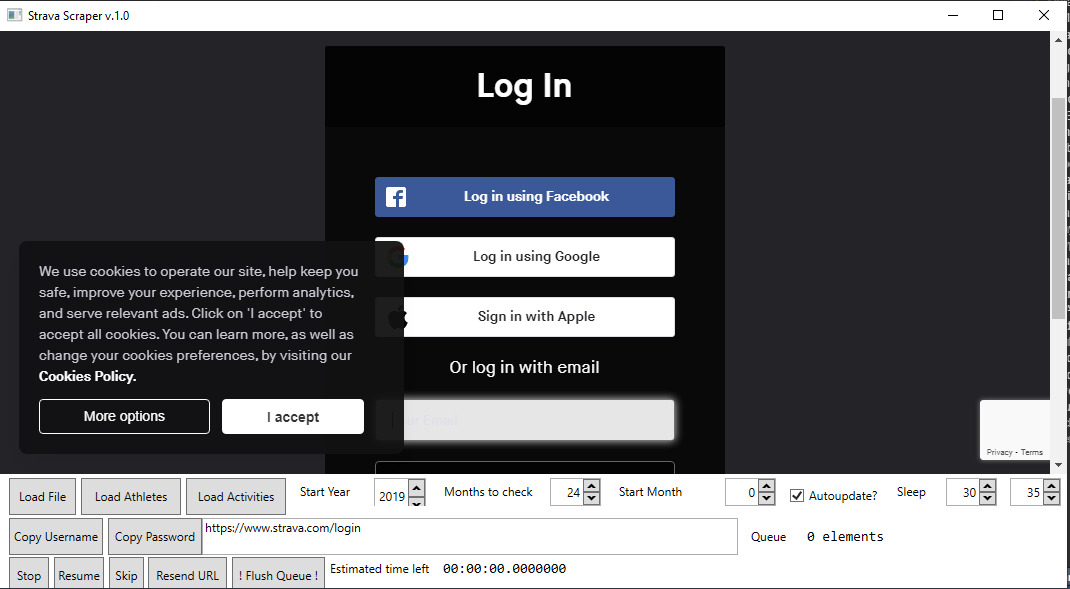
\includegraphics[trim=0in 0.01in 0.08in 0.05in,clip]{./includes/Strava_scraper.png}
\caption{The picture shows the user-interface of the Straver Scraper v.1.0}
\label{fig:scraper_pic}
\end{sidewaysfigure}
\clearpage


\includepdf[pages=-, pagecommand={}]{eidesstattliche_versicherung.pdf}



\end{document}
